\documentclass{article}
\usepackage{aaai}
\nocopyright
\usepackage{graphicx}
\usepackage[ruled, vlined, linesnumbered]{algorithm2e}
\usepackage[toc, page]{appendix}

% Big margins for now so people can take notes/scribbles.
%\usepackage{fullpage}

\title{Best-First Heuristic Search for Multi-Core Machines}
%\author{Ethan Burns \and Seth Lemons \and Wheeler Ruml \\
%  Department of Computer Science \\
%  University of New Hampshire \\
%  Durham, NH 03824 USA \\
%  \{eaburns,seth.lemons, ruml\}@unh.edu}
\author{Ethan Burns \\
  Department of Computer Science \\
  University of New Hampshire \\
  Durham, NH 03824 USA \\
  eaburns@unh.edu}
\date{\today}

\begin{document}
\maketitle

\begin{abstract}
  In this paper we build on some of the techniques used for external
  memory search to create a parallel best-first style search.  Our new
  search algorithm, called Parallel Best NBlock First (PBNF), can be
  used to more quickly solve smaller search domains.  The PBNF
  algorithm outperforms the state of the art parallel search
  techniques in one of the two domains which we examine.  Also, the
  design of our new algorithm allows it to be trivially adapted to
  parallelize a host of other algorithms such as sub-optimal,
  pessimistic or optimistic heuristic search.
\end{abstract}

\section{Introduction}

In the field of artificial intelligence it is always beneficial to
solve problems more quickly.  Chip manufacturers are no longer
creating processors with more hertz, and because of this AI
researchers must begin finding methods of using parallelism for speed.
For this work our goal was to use parallelism provided by multi-core
processors to solve heuristic search problems as fast as possible.

In a typical (serial) best-first search algorithm, an \emph{open-list}
and \emph{closed-list} of nodes are maintained.  The open-list
contains nodes on the search frontier that have yet to be searched
(expanded).  The open-list is usually sorted on the f-value for each
node, where $f(n)$ for a node $n$ is the estimated cost for a solution
path which goes through $n$.  The closed-list contains all nodes which
have already been searched, and it can be used to detect nodes which
have already been searched.  The process of detecting nodes that have
already been searched is called \emph{duplicate detection}.  In a
serial best-first search, a node is added to the closed-list the first
time that the search encounters it.  If a node is encountered again
during the search process (assuming that an admissible and consistent
heuristic is used) it can be ignored since it has already been
expanded.  This process breaks cycles and eliminates extra, wasted,
search effort.

One of the greatest challenges of parallel heuristic search is
reducing synchronization overhead.  This can be seen by looking at a
naive approach to parallelizing heuristic search where a global open
and closed list are used with a mutual exclusion lock (called a
\emph{mutex}) to prevent data races.  The problem with this approach
is that, as the number of processors increases, there will be an
increasing amount of contention on these two data structures.  This
will create a large bottleneck, greatly slowing down the search.  This
result can be seen in work done by Seth Lemons \cite{lemons:sur}

Various methods have been proposed that attempt to alleviate the
overhead of synchronizing the access to global data structures in
parallel heuristic search algorithms.  The problem with most of these
approaches is that they still require processors to lock a mutex
during the ``fast-path'' of the search -- while expanding nodes.
Other algorithms make use of depth-first or breadth-first search
instead of using a best-first ordering to reduce contention.  While
these methods may scale with more processors, they still suffer from
the brute-force nature of the depth-first and breadth-first search
methods.  Each of these techniques also suffers from additional
disadvantages: depth-first search performs \emph{very} poorly on
domains which have a lot of duplicates, and breadth-first search
performs poorly on domains which do not have unit cost edges.

The algorithm which is presented in this paper extends some ideas
which were developed for external memory search -- an area which
shares some of the same algorithmic design challenges as parallel
search.  Our algorithm, which is called Parallel Best NBlock First
(PBNF), enables processors to acquire exclusive access to sections of
a search space in a manner which allows for periods of
synchronization-free search.  Additionally, this method lets the
search progress in a best-first manner which detects duplicates and
can perform well in domains with non-uniform move costs.  Moreover
PBNF can be trivially adapted to use sub-optimal, weighted or
pessimistic heuristics.

We demonstrate the performance of our algorithm on two common search
domains, including grid-world and the sliding tiles domain.  Our
results show that this algorithm can outperform all algorithms which
we compare against.

\section{Previous Work}

Before describing our new algorithm, we will discuss a couple of other
parallel heuristic search algorithms.  In this section we also
describe some serial algorithms from which we gathered some of the
ideas for our new parallel approach.

\subsection{Parallel Retracting A*}

There have been a handful of algorithms created that attempt to
alleviate the amount of contention between processors performing
parallel heuristic search, by making use of distributed open and
closed lists instead of using global data structures.  One such
algorithm is Parallel Retracting A* (PRA*) \cite{evett:pra}.  In PRA*
a hashing scheme is used to divide the search nodes among all of the
available processors.  Each time a node is expanded it is passed to
the appropriate processor dictated by the hash function.  Each
processor is then in charge of expanding and detecting duplicates for
all of the nodes that hash to it.  This method allows duplicate
detection to happen without requiring all processors to track every
node which has been expanded (a process which often requires a large
amount of synchronization), it also reduces the amount of contention
on the open-list by distributing it amongst all of the
processors\footnote{The true PRA* algorithm also uses a
  node-retraction scheme to reduce the amount of memory that a search
  requires.  For this work, we are only concerned with searches that
  fit into memory, and our interest in PRA* is for its unique method
  of splitting the search space among processors, not its
  node-retraction scheme.}.

One of the problems that PRA* encounters is that, while no
synchronization is required for duplicate detection, there is a
substantial amount of overhead incurred by the message passing that is
used to move nodes to their respective processors.  In a shared memory
system, each processor must have a synchronized open-list which all of
the other processors have the ability to add search nodes to.  While
this is less of a bottle-neck than having a single global, shared
open-list, we have found that it is still very expensive.  Work done
by Seth Lemons in his survey of parallel heuristic search algorithms
\cite{lemons:sur} demonstrates that the performance for PRA* suffers
from the overhead of passing nodes to their respective processors.

\subsection{Structured Duplicate Detection}

Structured Duplicate Detection or SDD \cite{zhou:sdd} is a method for
performing external memory search.  SDD uses a projection function, a
many-to-one mapping from states in a search space to states in an
abstract space, to decompose a search graph.  The projection function
creates an abstract space of nodes that are projections, or images, of
the nodes in the original state space.  Since the projection function
is a many-to-one mapping, the abstract space is significantly smaller
than the original search space.  For a projection function $p$, $y$ is
said to be the \emph{image} of a node $x$ if $p(x) = y$.  Additionally
$y'$ is a successor of $y$, in the abstract graph, if there are two
states $x$ and $x'$ such that $x'$ is a successor of $x$, $y$ is the
image of $x$ and $y'$ is the image of $x'$.  In other words:
\begin{eqnarray*}
  &&x' \in successors(x) \wedge p(x) = y \wedge p(x') = y'\\
  &&\Rightarrow y' \in successors(y)
\end{eqnarray*}
In the description of the SDD algorithm, Zhou and Hansen use the term
\emph{nblock} to refer to all nodes in the original state space that
have the same image in the abstract space.  Throughout the remainder
of this paper, the terms ``abstract state'', and ``nblock'' will be
used interchangeably, as each nblock corresponds to a single abstract
state.

Zhou and Hansen show that while performing duplicate detection with
SDD, only nodes which reside within the same nblock must be consulted.
This is because, for a node $x$ which is a duplicate of a node $z$,
both $x$ and $z$ will project to the same abstract state (and
therefore reside in the same nblock) Intuitively, this makes sense,
because both $x$ and $z$ are the same node since they are duplicates.
This leads to the idea of a \emph{duplicate detection scope}.  By the
definition of the successor set of an abstract node, any child node
$x'$ of a node $x$, in the original state space, will have an image
$p(x') \in successors(p(x))$, and therefore when performing duplicate
detection for $x'$ the only nodes that must be checked are in the
nblock $p(x') \in successors(p(x))$.  For this reason,
$successors(p(x))$ is called the duplicate detection scope of the
nblock $p(x)$ -- no other nodes in the original state space will ever
need to be consulted for duplicate detection when expanding nodes in
the nblock $p(x)$.

This idea can be illustrated using the sliding tile puzzle as an
example.  One possible projection function for the sliding tiles
puzzle would be to only look at the position of the empty tile.  For
example: all states with the empty tile in the upper left-hand corner
(position 0) would map to the nblock shown on the left in Figure
\ref{fig:tile-abstraction}, where the grayed square represents the
position of the empty tile.  Using this abstraction, there are sixteen
possible abstract states, one for each possible position of the empty
tile.  It is easy to see that all of the children of a state in the
nblock shown on the left in Figure \ref{fig:tile-abstraction} will
have the empty tile in either position 1 or 4 (either by sliding the
tile in position 1 to the left, or by sliding the tile in position 4
up).  The diagram on the right, in Figure \ref{fig:tile-abstraction},
shows the duplicate detection scope for the nblock shown on the left
in this figure.  Any of the children of a state in the nblock shown on
the left in Figure \ref{fig:tile-abstraction} will fall into one of
the two nblocks shown on the right.

\begin{figure}[t]
  \begin{center}
    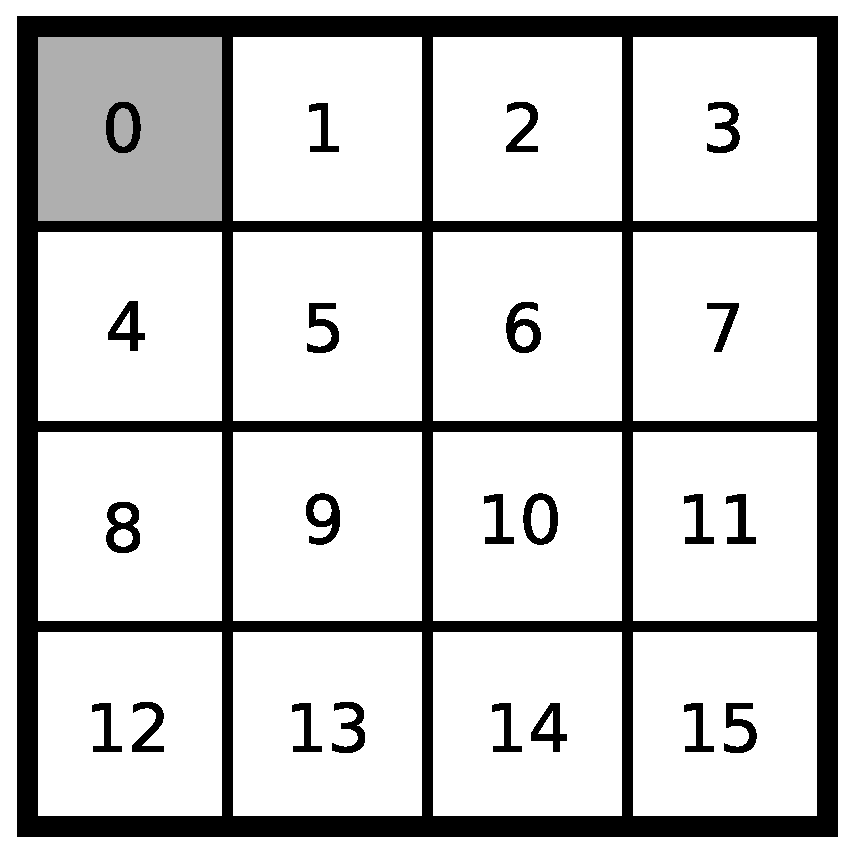
\includegraphics[width=1in]{images/tile-abstraction.eps}
    \hspace{1cm}
    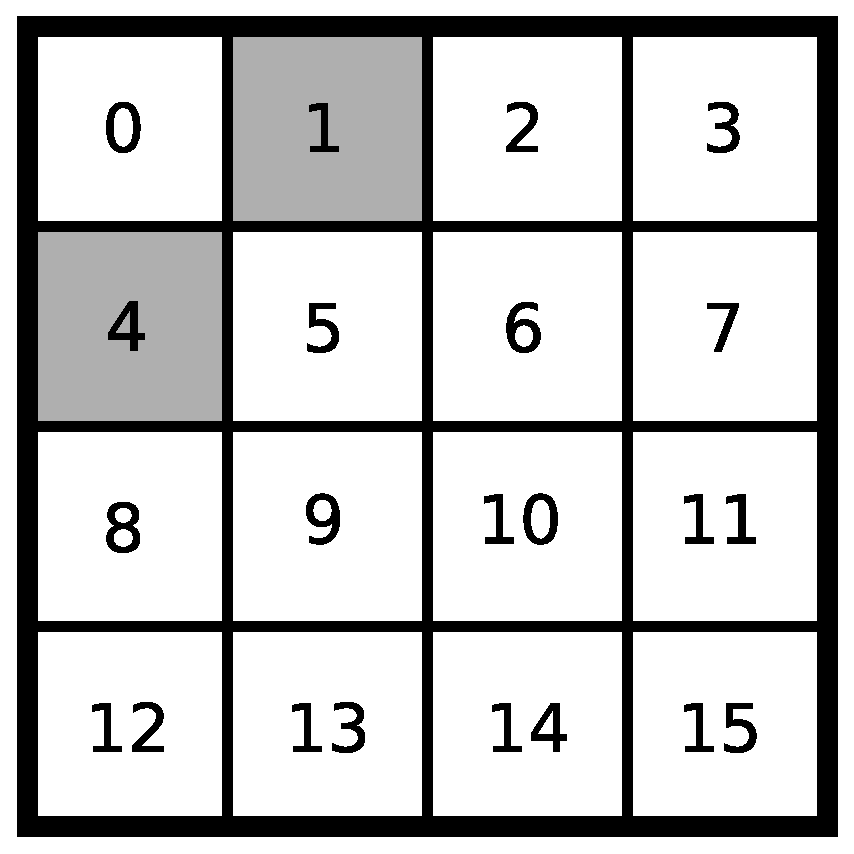
\includegraphics[width=1in]{images/duplicate-detection-scope.eps}
    \caption{The abstract image of all states with a empty tile in
      position 0 (left).  The duplicate detection scope of the
      abstract state with the empty tile in position 0 (right).}
    \label{fig:tile-abstraction}
  \end{center}
\end{figure}

The main focus of the SDD approach is: using state space decomposition
so that generated nodes can be explicitly moved to a secondary storage
device (such as a disk drive) when they are not in the duplicate
detection scope of the nblock being expanded.  The SDD approach uses
breadth-first heuristic search \cite{zhou:bhs}, where only the nodes
of the current search depth in a single nblock are searched at a time.
Nodes of this nblock are expanded from the current depth-layer and
their children are placed into the next-depth layer of their
corresponding nblocks.  When the current nblock has no more nodes at
the current depth-layer, it is swapped for another nblock which does
have open nodes at this depth.  If no more nblocks have nodes at the
search depth, the search progresses to the next layer (which contains
the children nodes of the previous layer).  This procedure repeats
until a goal is found, or until no nodes remain. Since duplicates can
only fall into the duplicate detection scope of the nblock being
searched, the remainder of the nodes can be pushed off to disk,
instead of being stored in main-memory.  Nblocks can then be
intelligently swapped into and out of main-memory as the search
progresses.

\subsection{Parallel Structured Duplicate Detection (PSDD)}

While the motivation of SDD is to have explicit control over which
portions of a search space reside in main-memory.  Zhou and Hansen
also show that this approach lends itself to parallelization
\cite{zhou:psd}.  The parallel SDD (or PSDD) algorithm uses the graph
of nblocks to find \emph{disjoint duplicate detection scopes}, or
duplicate detection scopes that do not overlap.  Nblocks with disjoint
duplicate detection scopes can be searched in parallel without any
locking or contention.  In order to find nblocks with disjoint
duplicate detection scopes the concept of a \emph{free} nblock is
introduced.  An nblock $b$ is considered to be free if no processor
has acquired an nblock in $successors(b)$ -- in other words, if all
other processors are searching nblocks with duplicate detection scopes
which are disjoint from that of $b$.  Free nblocks are found by
tracking a $\sigma(b)$ value for each nblock $b$, where $\sigma(b)$ is
the number of nblocks in $successors(b)$ that are in use by another
processor.  Any nblock $b$ with $\sigma(b) = 0$ is free, and therefore
a processor can acquire $b$ and its duplicate detection scope for a
period of lock free expansion.  Besides tracking disjoint duplicate
detection scopes, the search procedure of PSDD is the same as that of
SDD; the search progresses by searching one depth-layer at a time
until a goal is found or the search space is exhausted.

PSDD is an attractive algorithm because it reduces the amount of
contention between processors by allowing for lock-free periods of
expansion.  The only lock used in the PSDD algorithm is used when
finding a new free nblock to search.  The problem with the PSDD
approach, however, is that it performs a breadth-first style of search
which only makes weak usage of the heuristic estimate of a node, and
requires all of the processors to synchronize between each layer.
Furthermore because of the breadth-first nature of PSDD, the algorithm
will not perform well on domains which do not have unit-cost moves.
This is because, in such a domain, each layer of the search may have
only a small number of new nodes.  If there are not enough nodes in a
layer to amortize the cost of synchronizing all of the processors
between layers, or worse if there are not enough nodes to keep all
processors busy, then the search will perform very poorly.

\subsubsection{Best-First PSDD}

Typically the PSDD algorithm uses breadth-first search because it can
be made more memory efficient than a typical best-first search
\cite{zhou:bhs}.  Since PSDD was created to solve very large problems,
memory efficiency is beneficial even with the use of external storage
(for example, I/O operations can be smaller and less frequent).
Without an upper bound on the solution cost, however, breadth-first
search can be rather brute-force and inefficient.  Zhou and Hansen
suggest a modification to the SDD (and PSDD) algorithm to make the
search use a best-first order \cite{zhou:sdd} (we call this modified
PSDD algorithm BFPSDD for best-first PSDD).  This modification
performs a layer-by-layer search like SDD and PSDD but, in this case,
each layer consists of all of the nodes with the same f-value.  The
BFPSDD algorithm stores all nblocks in a heap which is sorted by the
best f-value of the best node in each nblock.  At every layer, BFPSDD
populates its list of free nblocks with all of the nblocks which have
the next best f-value on the heap.  When searching an nblock, a
processor searches all of the nodes in the nblock which have an
f-value equal to the current layer's f-value.  Once all of the nodes
with a given f-value are searched, all of the processors synchronize
and the search progresses to the next f-value layer by re-populating
the free list with all nblocks from the heap that have the next best
f-value.  It is easy to see that this search will progress in a
best-first manner.

\subsection{Localizing A*}

An alternative approach to external memory search for improving
efficiency in large search spaces is to slightly loosen the node
ordering restriction of A* as is done by Edelkamp and Schrodl
\cite{edelkamp:loc}.  Edelkamp and Schrodl present an algorithm that
uses a looser node ordering than A* in order to achieve better memory
locality. We refer to this algorithm as LA* (for localized A*).  While
LA* expands more nodes than A* does, the intuition is that LA* can
achieve better performance than A* for large searches because it can
reduce the number of virtual-memory operations that swap to disk.

LA* uses a data structure called a \emph{heap-of-heaps} to order its
node expansions.  A heap-of-heaps, $H$, is composed of elements
$H_0$,$H_1$,...,$H_n$ where each element $H_i$ is a heap of search
nodes that reside in the same page of memory.  The heap-of-heaps, $H$,
is loosely sorted on the f-values of the best node of each heap $H_i$
(denoted as $best(H_i)$).  The LA* procedure searches the best heap
$H_0$, of the heap-of-heaps, until $best(H_1) + \Delta > best(H_0)$,
where $H_1$ is the new best heap on $H$ after the removal of $H_0$.
The $\Delta$ value allows the search to expand a set of nodes in $H_0$
which may not have the best f-values, but that have better memory
locality with respect to the previously expanded nodes.

Since LA* tends to prefer nodes with better memory locality, it can
reduce the number of page-faults, and virtual memory swap operations
that the operating system must perform.  The tradeoff is that the
first solution found by LA* may be sub-optimal since it is not
searching in strict best-first order.  To fix this problem, LA*
doesn't return its first solution, instead it behaves like an anytime
search algorithm by continuing the search and pruning on the f-value
of incumbent solutions \cite{hansen:ahs}.  Since the f-value of an
incumbent solution is an upper-bound on the optimal solution, the
search can stop when there are no frontier nodes that have f-values
less than the current incumbent -- this means that the current
incumbent solution is the optimal solution.

\section{Parallel Best NBlock First (PBNF)}

In order to get the benefits of lock-free expansion and duplicate
detection which are provided by the PSDD algorithm, without the need
for layer-synchronization, we have created an algorithm that combines
the ideas from PSDD and LA* which we call Parallel Best NBlock First
(PBNF).  The PBNF algorithm uses a state space projection function and
maintains a heap of free nblocks where each nblock has a heap of open
nodes sorted on f-value and a hash table of closed nodes which have
already been searched.  Processors use the heap of free nblocks to
attempt to acquire the free nblock with the best open node.  A
processor will search its acquired nblock as long as it contains nodes
which are better than those of the nblock on the front of the heap of
free nblocks.  If the acquired nblock becomes worse than the best free
nblock, the processor will attempt to release its current nblock and
acquire the better one.

\begin{algorithm}
  \caption{PBNF Search}
  \SetKwData{block}{b}
  \SetKwData{node}{n}
  \SetKwData{incumbent}{incumbent}
  \SetKwData{children}{children}
  \SetKwData{child}{c}
  \label{alg:pbnfsearch}
  \KwResult{Searches nblocks for a goal node.  After each process
    completes, \incumbent contains the optimal solution.}
  \Repeat{$\forall i \in Nodes : f(i) > f(incumbent)$} {
    $\block \leftarrow$ acquire best free nblock\;
    \While {$\block$ is better than the next best free nblock} {
      $\node \leftarrow$ best node on $\block$\;
      \If {$\node$ is a goal}{
        \If{$f(\node)$ < $f(\incumbent)$}{
          $\incumbent \leftarrow$ $\node$\;
        }
      }
      \Else {
        $\children \leftarrow$ expand $\node$\;
        \ForEach{$\child \in \children$}{
          place $\child$ in its appropriate nblock\;
        }
      }
    }
  }
\end{algorithm}

Algorithm \ref{alg:pbnfsearch} gives a general overview of the search
procedure that is performed by each process in PBNF.  Each process
greedily acquires a free nblock from the heap of free nblocks and
searches it while it remains better than the new best free nblock.
There is no layer synchronization, so it is possible that the first
solution found is suboptimal.  Since we are interested in optimal
solutions, a global incumbent solution is kept and used for pruning
the open list.  Like LA*, when all of the nodes have been pruned, the
incumbent solution is the optimal solution which will then be returned
by the search procedure.

Each time a processor expands a node off of its acquired nblock, it
must test the head of the heap of free nblocks to see if it is still
looking at better nodes in its acquired nblock.  Since it is possible
that an nblock has only a very small number of nodes which are better
than the next free nblock, PBNF implements a simple scheme to reduce
the amount of nblock switching.  When a processor acquires a new
nblock for expansion, it is required to search at least a minimum
number, $m$, nodes off of the nblock before it considers switching.
This is done as an attempt to reduce the contention on the nblock
heap.  Without requiring $m$ expansions before switching nblocks, we
anticipate that there will be too much contention on the heap of free
nblocks when many nblocks have similar quality nodes.  Our
experimental results seem to agree with this observation.

In addition to the parameter $m$, the PBNF algorithm attempts to
reduce the amount of time that a processor is waiting on a mutex by
using a \texttt{try\_lock} operation when ever possible.  A
\texttt{try\_lock} operation attempts to gain exclusive access to a
mutex, however, if it fails it returns a failure instead of putting
the calling process to sleep until the mutex is available.  In
situations when a processor is trying to acquire a new nblock, but the
current nblock has nodes remaining in its open list the
\texttt{try\_lock} can be used.  If the \texttt{try\_lock} fails, the
processor can expand more nodes off of its current nblock instead of
sleeping.  These nodes may not be very good (that is why the processor
was switching in the first place), but this is still much more
beneficial than sleeping.  Were the \texttt{try\_lock} not used, the
processor would be doing \emph{nothing} while waiting for the lock
instead or expanding some nodes which may not be good now, but that
may need to be searched later anyway.

One of the most important features of the PBNF algorithm is that it is
simply a parallel version of best-first search.  The basic algorithm
that we have presented here sorts nodes based on their f-values, but
instead nodes can be sorted in a variety of other parameters leading
to a host of other parallel search algorithms.  A weighted or
pessimistic heuristic can be used to provide a parallel sub-optimal
search (this would also require the removal of the any-time portion of
the algorithm which guarantees optimality).  Additionally it would be
trivial to modify PBNF to produce a parallel, optimistic sub-optimal
search \cite{thayer:fas}.  It is easy to imagine lots of other
modifications too.  Although we have not yet explored any of these
flavors of PBNF, we believe that they could be greatly beneficial and
should be explored in the future.

\subsection{Safe PBNF}

One problem with PBNF is that the greedy free-for-all order in which
processors acquire free nblocks can lead to a live-lock in domains
with infinite state spaces.  It is possible to show an order which
nblocks are acquired and released such that some nblocks are never
added to the free list.  If the goal resides on one of these nblocks
and the search space in not finite, the search may never complete.  To
fix this issue, we have developed a method where processors
voluntarily release the nblock which they are expanding if they are
interfering with a better nblock.  We call this modified version of
PBNF, ``safe PBNF.''

In the safe PBNF algorithm, a processor periodically checks the
nblocks which it is preventing from becoming free (we call these
blocks the \emph{interference scope} of an nblock) to see if any of
these nblocks are better.  This test happens each time a processor
checks the heap of free nblocks -- it happens each expansion after the
required $m$ expansions are performed.  If a processor finds a better
nblock in its interference scope, it flags this nblock as hot.  For
each nblock $b$ a value $\sigma_h(b)$ tracks the number of nblocks in
the interference scope of $b$ which are flagged as hot.  If
$\sigma_h(b) \neq 0$ the nblock $b$ is removed from the heap of free
nblocks.  This ensures that a processor will not acquire an nblock
which is preventing a hot nblock from becoming free.  Removing all
nblocks with $\sigma_h \neq 0$ from the nblock heap ensures the
property that if an nblock is flagged as hot it will eventually become
free.

Since processors can be searching nblocks with a wide range of
f-values, we also allow for a processor to un-flag a hot nblock
(setting it back to \emph{cold}).  This occurs when a processor finds
an nblock in its interference scope flagged as hot which is not better
than its current nblock.  In this case, it is not desirable for the
processor to relinquish its nblock, since it is better than the nblock
which is labeled as hot.  When this situation arises, the processor
which is not going to relinquish its nblock will set the hot nblock
back to cold and update the $\sigma_h$ values as appropriate, possibly
re-adding blocks to the free heap too.

A complete pseudo-code for the safe PBNF algorithm can be found in the
appendix.

\section{Experimental Results}

This section presents experimental results which compare PBNF to a
handful of other state of the art parallel heuristic search
algorithms.  The algorithms chosen for these experiments were the ones
that performed the best in the survey done by Seth Lemons on parallel
heuristic search \cite{lemons:sur}.  These algorithms were programmed
in C++ and make use of the POSIX threading library for concurrency.
For these experiments two domains are used, grid world path planning
and the sliding tiles puzzle.  All of the experiments in this section
were performed on dual quad-core Intel Xeon E5320 1.86GHz processors,
with 16Gb RAM running the 64-bit Fedora 9 operating system.

%% Mention how we only show results with PBNF and the PSDD-variations
%% due to experimental results from Seth's unpublished paper.

\subsection{Grid World Path Planning}

In the grid world path planning domain the goal is to find a path from
a start state $S$ to a goal state $G$ in a 2-dimensional grid.  To
complicate the problem, squares of the grid have a probability $P$ of
being obstructed, where a valid path can not include any obstructed
states.  We use two cost models, the unit cost model in which each
move has a cost of one, and the life cost model where moves have a
cost of the row number of the state where the move was performed.  In
this model, moves near the top of the grid are less expensive (row
zero is actually free) than the states near the bottom, and the most
direct path from the start to the goal may not be the least cost path.

The projection function which we used for the grid world domain
projects from a search state to an abstract state that only considers
the row of the search state modulo a value $M$.  The parameter $M$ can
be tuned to change the number of abstract states.  The number of
abstract states has the potential to greatly influence the performance
of the search.  If there are too many abstract states (and therefore
nblocks) then nblocks will be filled with only a very small number of
nodes and processors will be forced to switch after an insignificant
amount of searching.  If there are too few nblocks then there may not
be enough disjoint duplicate detection scopes and not all processors
will be able to search in parallel (instead they will be waiting on
free nblocks).

We hypothesized that the desired number of nblocks was related to the
number of processes that would be performing the search.  This is
because if more processes are searching more nblocks are required to
create a sufficient number of disjoint duplicate detection scopes.  If
fewer processes are searching, however, fewer scopes may be desired to
ensure that each nblock has a sufficient number of nodes.  We used the
parameter $M$ (which dictates the total number of nblocks for a grid
search) along with the number of searching processes to explore the
best setting for the number of \emph{nblocks per thread}.  The full
set of data for this mini-experiment is available in the appendix
along with another mini-experiment to find the best setting for the
parameter $m$ (minimum expansions per nblock) for PBNF.  In this
section of the paper, we present our results with the best combination
of parameters according to the data shown in the appendix for each
algorithm.

\subsubsection{Unit Cost}

\begin{figure}[t]
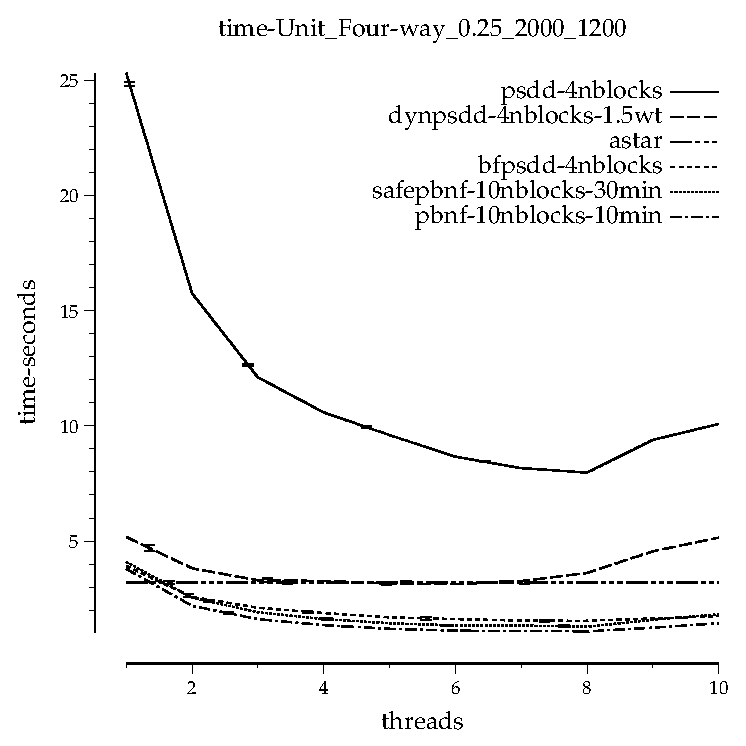
\includegraphics[width=3in]{images/grid-time-unit-fourway-025-2000-1200}
\caption{CPU time versus number of threads on a 2000x1200 unit-cost
  grid world with a 25\% probability that a square is obstructed.}
\label{fig:grid-unit}
\end{figure}

Figure \ref{fig:grid-unit} shows the performance of three flavors of
the PSDD algorithm along with PBNF and the Safe PBNF algorithms.  The
x-axis is the number of threads of execution\footnote{In our results
  we use the term threads instead of the term processes (which is used
  throughout the beginning of this paper) to be specific about this
  detail of our implementation.} for each search, and the y-axis
represents the average wall-clock time in seconds that each search
took to complete. The line labeled ``psdd-4nblocks'' shows the average
search time for the PSDD algorithm to solve a set of grid world
problems with four nblocks per thread.  The next line, labeled
``dynpsdd-4nblocks-1.5wt,'' shows the time for: a serial weighted A*
search with a weight of 1.5 followed by a PSDD search with pruning on
the solution cost from the previous weighted A*.  We call this
algorithm DYNPSDD (dynamically cost bounded PSDD) and we feel that
this may be a more reasonable demonstration of the performance of the
standard PSDD algorithm since the breadth-first search which PSDD uses
relies on upper-bound solution cost pruning.  The next set of data in
this plot is labeled ``bfpsdd-4nblocks,'' and it shows the performance
of the best-first flavor of the PSDD algorithm with four nblocks per
thread.  The final two data sets show the performance for safe PBNF
and PBNF with 10 nblocks per thread and 30 and 10 minimum expansions
per nblock respectively.

The first thing that this plot demonstrates is that the performance of
the PBNF algorithm is superior to that of the PSDD variants on these
instances of the unit-cost grid world domain.  The confidence
intervals shown in this plot are very tight; showing that the results
are indeed statistically significant.  The PBNF algorithm outperforms
all of the other algorithms, including the safe variant of PBNF.  We
suspect that the small amount of extra overhead incurred by safe PBNF
is from checking the interference scopes for nblocks to label as hot,
and because removing nblocks which interfere with hot nblocks from the
nblock heap makes for slightly fewer free disjoint duplicate detection
scopes.  The ``good parameter settings'' for the safe PBNF algorithm
help to back up our suspicion.  Safe PBNF performs best with a larger
number of required minimum expansions per nblock than standard PBNF.
By performing more expansions before testing the interference scope of
the acquired nblocks, the overhead is slightly reduced.

As mentioned at the beginning of this section, the computers used to
run these experiments have a total of eight cores.  This means that
the machines which performed these searches should, ideally, show
improved performance by increasing the thread count up to eight (one
thread for each core).  A more subtle -- but equally important --
observation from this plot is that the DYNPSDD algorithm begins
performing slightly worse as more threads are added.  While all of the
other algorithms perform better as more threads are added, the DYNPSDD
algorithm seems to perform increasingly worse as more threads are
added beyond six.  One reason for this may be because the cost of the
serial weighted A* search becomes the limiting factor preventing the
search from taking full advantage of the parallelism from the PSDD
portion.  The problem with this explanation is that it only accounts
for why DYNPSDD doesn't perform \emph{better} as threads are added,
not why it begins to perform slightly worse.  This issue is still open
for future exploration.

\subsubsection{Life Cost}

\begin{figure}[t]
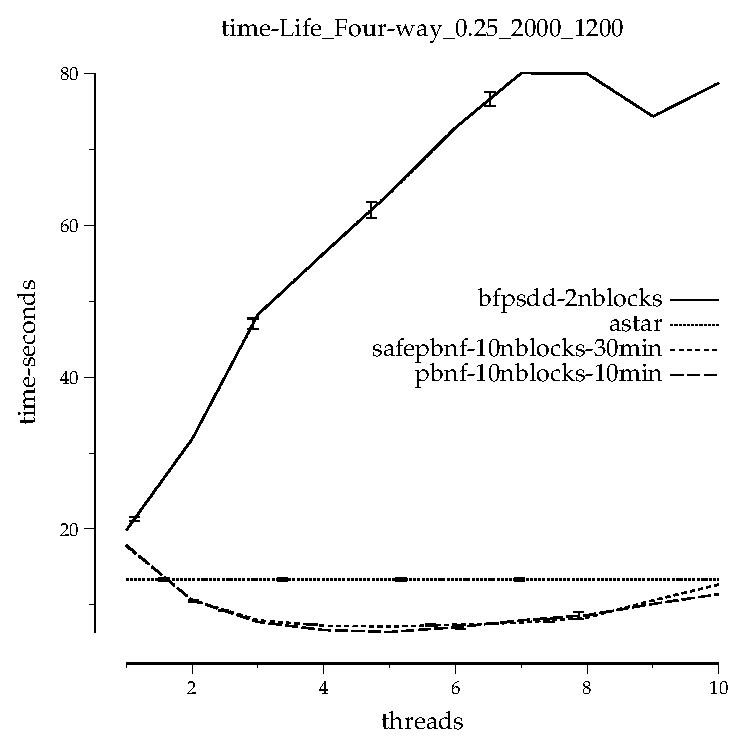
\includegraphics[width=3in]{images/grid-time-life-fourway-025-2000-1200}
\caption{CPU time versus number of threads on a 2000x1200 life-cost
  grid world with a 25\% probability that a square is obstructed.}
\label{fig:grid-life}
\end{figure}

Figure \ref{fig:grid-life} shows the performance of the best-first
PSDD algorithm along with the two PBNF algorithms on life-cost
boards.  The standard PSDD and DYNPSDD algorithms are not shown here
since the breadth-first search which they use is not designed for
non-unit cost domains.

Figure \ref{fig:grid-life} shows that the PBNF algorithms greatly
outperform best-first PSDD in the life cost grid domain.  The reason
why best-first PSDD doesn't perform well on this domain is because
there are many cost layers which may contain only a small number of
search nodes.  This means that best-first PSDD will perform a large
number of synchronizations with only a small amount on searching
in between.  Since the PBNF algorithm doesn't use layer-based
synchronization, it continues to perform well on the life-cost grid
world boards without modification.

Another aspect of this plot that is notable is that all of the
algorithms show a performance decrease as more threads are added.  One
reason why the best-first PSDD shows a decreased performance is
because the synchronization steps are more expensive since there are
more threads to synchronize.  For PBNF, however, it is not quite as
obvious why the performance decreases.  We suspect that this is
because of the projection function which we use.  As previously
mentioned, the projection function that we use for the grid world
domains only looks at the row of a grid state.  In the life cost grid
instances, the cost of a move is the same as the row number from which
the move was executed.  This means that it is often best to move
straight up to the top of the grid, across the free row-zero and then
down to the goal.  It is possible that, since the search progresses
up-then-down the grid, instead of across, that nblocks only have a
small number of nodes.  In future work different projection functions
should be explored, we suggest:
\begin{enumerate}
\item Only look at columns.
\item Look at both columns and rows of the search space, but use a
  coarser grid in the abstract space.  For example, the grid world
  instance shown in Figure \ref{fig:small-grid}, could be decomposed
  into two abstract states, one which contains squares: (0,A), (0,B),
  (1,A) and (1,B) and another which contains squares: (0,C), (0,D),
  (1,C) and (1,D).
\end{enumerate}

\begin{figure}[t]
\begin{center}
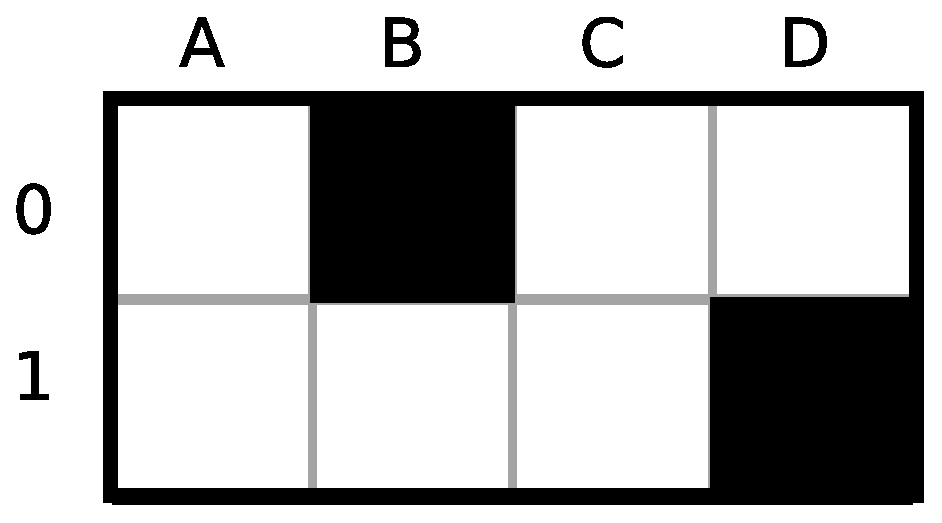
\includegraphics[width=3in]{images/grid-world-small.eps}
\caption{A 7x2 grid world}
\label{fig:small-grid}
\end{center}
\end{figure}

\subsection{Sliding Tiles}

The sliding tiles puzzle is a common domain for benchmarking heuristic
search algorithms.  In this paper we use 7x2 sliding tiles puzzles
(13-puzzles) because they are small enough to fit into memory, but are
difficult enough that the timing measurements can be accurate.

The projection function which was used for these puzzles was similar
to the one shown in Figure \ref{fig:tile-abstraction}, except instead
of using just the position of the blank tile, the projection takes
into account the position of the 1-tile too.  This make for 182
abstract states.  Using this projection function there is no
parameter, like the $M$ parameter for grid world which can control the
number of nblocks, so the nblocks per thread value is not displayed
for these plots, as the number of nblocks remains constant at 182.

Figure \ref{fig:tiles-7x2} shows the performance of the best-first
PSDD algorithm and the two PBNF algorithms on a set of 7x2 sliding
tiles puzzles.  Due to the large variance in the difficulties of these
problems the y-axis of Figure \ref{fig:tiles-7x2} shows the solution
time normalized to that of a serial A*.We can see in this figure that,
as the thread count increases the best-first PSDD algorithm performs
significantly better than the PBNF algorithms.  In fact, BFPSDD gets
increasingly better as threads are added, but PBNF gets significantly
worse with more than three threads and safe PBNF performs better as
threads are added until six, then its performance decreases with
additional threads.  One reason for this is that, as the number of
threads increases, there may not be enough disjoint duplicate
detection scopes to keep all of the threads searching at once.  This
theory can be partially supported by the fact that the best minimum
expansions parameter settings for the two PBNF algorithms is
relatively high compared to that of the grid world domain.  This means
that more expansions are required to reduce the great amount of
contention on the heap of free nblocks.  This hypothesis is also
supported by the fact that both the PBNF and safe PBNF algorithms do
improve in performance up to a point, it would seem that this point is
when contention becomes overwhelming.

\begin{figure}[t]
\begin{center}
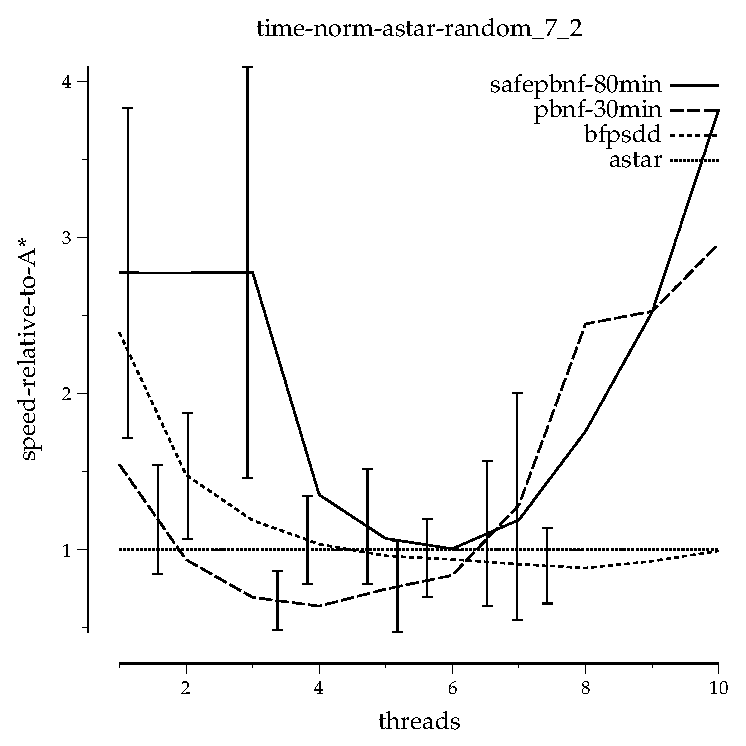
\includegraphics[width=3in]{images/tiles-time-norm-random-7-2.eps}
\caption{Search time relative to A* versus number of threads on a set
  of 7x2 sliding tiles puzzles using the blank, 1-tile for the
  projection function.}
\label{fig:tiles-7x2}
\end{center}
\end{figure}

\begin{figure}[t]
\begin{center}
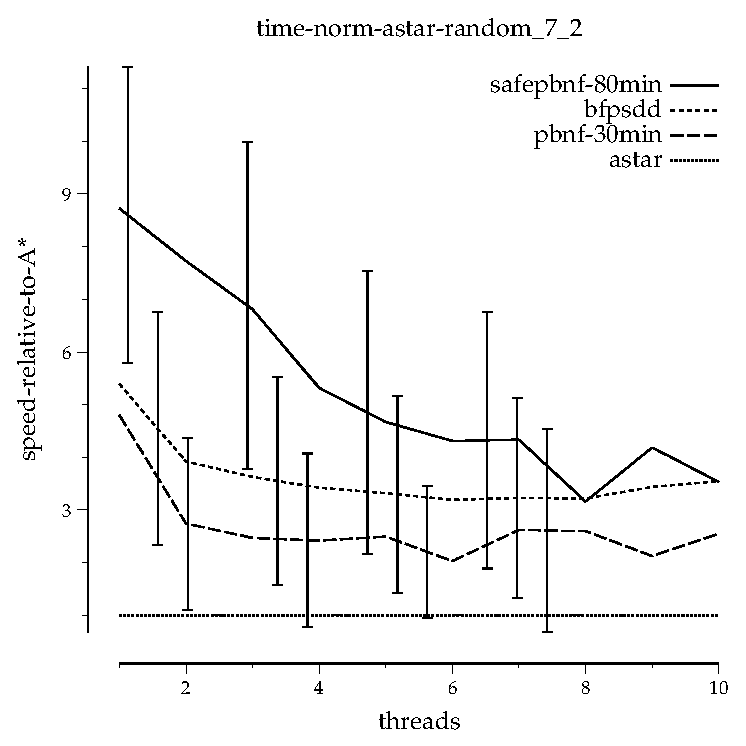
\includegraphics[width=3in]{images/tiles-time-norm-random-7-2-newabstraction.eps}
\caption{Search time relative to A* versus number of threads on a set
  of 7x2 sliding tiles puzzles using the blank, 1-tile and 2-tile for
  the projection function.}
\label{fig:tiles-7x2-new}
\end{center}
\end{figure}

We speculate that, to correct this problem, a larger abstract state
space could be used to create more nblocks.  Future work should
explore the projection function that tracks the blank tile, 1-tile and
2-tile.  This would create 2184 nblocks, which should create a
sufficient number of disjoint duplicate detection scopes.

\section{Conclusion}

We have presented a new parallel heuristic search algorithm (PBNF)
which makes use of some techniques traditionally used in external
memory search to solve search problems more quickly.  The PBNF
algorithm attempts to use a best-first search ordering without
layer-synchronization, and because of this it is trivial to adapt PBNF
to perform many other algorithms in parallel, including: weighted,
pessimistic and optimistic heuristic search.  In addition, we have
performed an analysis of the performance of the PBNF algorithm along
with the PSDD algorithm, which has been shown to be the nearest
competitor for PBNF on the chosen domains.  In all of the grid world
domains the PBNF algorithm outperforms all of the variants of the PSDD
algorithm.  When solving the tiles puzzle, however, the PBNF algorithm
begins to perform worse as more search threads are added.  We believe
that this is because of a flaw in our projection function, and not the
algorithm.  This problem is still open for debate and future research.

\section{Acknowledgements}
We gratefully acknowledge support from NSF grant IIS-0812141.  We
would like to acknowledge and thank Seth Lemons, Wheeler Ruml, Rong
Zhou, for devoting a large amount of time to helping develop and test
the PBNF algorithm.  We would also like to thank Jordan Thayer for
help with suggestions on this paper.

\bibliography{master}
\bibliographystyle{aaai}

\begin{appendices}
\section{Pseudo Code}
%
% Include this file in a .tex document with \usepackage{algorithm2e}.
%

\SetKwData{block}{block}
\SetKwData{init}{init}
\SetKwData{incumbent}{incumbent}
\SetKwData{open}{open}
\SetKwData{closed}{closed}
\SetKwData{FreeList}{FreeList}
\SetKwData{minexpansions}{minexpansions}
\SetKwData{expansions}{expansions}

\SetKwFunction{threadsearch}{threadsearch}
\SetKwFunction{hot}{hot}
\SetKwFunction{interferenceScope}{interferenceScope}
\SetKwFunction{isfree}{isfree}
\SetKwFunction{setcold}{setcold}
\SetKwFunction{release}{release}
\SetKwFunction{sethot}{sethot}
\SetKwFunction{best}{best}
\SetKwFunction{shouldswitch}{shouldswitch}
\SetKwFunction{nextnblock}{nextnblock}

\begin{function*}
  \caption{search(init)}
  \KwIn{\init -- the initial node}
  \KwOut{The optimal solution, or NULL if no solution is found}
  insert \init into \open of the appropriate nblock\;
  insert \init into \closed of the appropriate nblock\;
  \lForEach{Processor}{$\threadsearch()$\;}
  \lWhile{any thread is still running}{wait\;}
  \Return incumbent
\end{function*}

\begin{function*}
  \caption{threadsearch()}
  \SetKwData{node}{node}
  \SetKwData{children}{children}
  \SetKwFunction{expand}{expand}

  \KwResult{Sets \incumbent if a solution is found}

  $\block \leftarrow$ NULL\;
  \While {{\bf not} done} {
    $\block \leftarrow \nextnblock(\block)$\;
    $\expansions \leftarrow 0$\;
    \While {{\bf not} $\shouldswitch(\block,\expansions)$} {
      $\node \leftarrow$ next node in \block\;

      \lIf {$\node > \incumbent$} {
        prune \node\;
      }

      \If {\node is a goal}{
        \lIf {$\node < \incumbent$}{
          $\incumbent \leftarrow \node$
        }
      }

      \ElseIf {\node is not a duplicate}{
        $\children \leftarrow$ \expand(\node)\;
        insert \children into \open of the appropriate nblock\;
      }

      $\expansions \leftarrow \expansions + 1$\;
    }
  }
\end{function*}

\begin{function*}
  \caption{isfree(block)}
  \KwIn{\block -- an nblock}
  \KwOut{Whether or not the given nblock is free}
  \Return $\sigma(\block) = 0$ {\bf and} $\sigma_h(\block) = 0$
          {\bf and} \block is not empty\;
\end{function*}

\begin{function*}
  \caption{shouldswitch(block, expansions)}
  \KwIn{\block -- an nblock to search,\\
    \expansions -- the number of nodes expanded in \block so far}
  \KwData{\minexpansions -- the minimum number of expansions to
    perform per-nblock}
  \KwOut{Whether or not the nblock should be switched}

  \lIf{\block is empty}{
    \Return true\;
  }
  \lIf{$\expansions < \minexpansions$}{
    \Return false\;
  }
  \If{$\best(\FreeList) < \block$ {\bf or}
    $\best(\interferenceScope(\block)) < \block$}{
    \If{$\best(\interferenceScope(\block)) < \best(\FreeList)$} {
        $\sethot(\best(\interferenceScope(\block)))$\;
    }
    \Return true\;
  }
  \ForEach{$b' \in \interferenceScope(\block)$}{
    \lIf{$\hot(b')$}{
      $\setcold(b')$\;
    }
  }
  \Return false\;
\end{function*}

\begin{function*}
  \caption{sethot(block)}
  \KwIn{\block -- an nblock}
  \KwResult{\block is flagged as hot}
  \If{{\bf not} $\hot(\block)$ {\bf and} $\sigma(\block) > 0$ {\bf
  and} $\neg\exists i \in interferenceScope(\block) : i < \block \wedge \hot(i)$ }{
    $\hot(\block) \leftarrow true$\;
    \ForEach{$n' \in \interferenceScope(\block)$}{
      \lIf{$\hot(n')$} {
        $\setcold(n')$\;
      }
      \lIf{$\isfree(n')$}{
        $\FreeList \leftarrow \FreeList \setminus \{n'\}$\;
      }
      $\sigma_h(n') \leftarrow \sigma_h(n') + 1$\;
    }
  }
\end{function*}

\begin{function*}
  \caption{setcold(block)}
  \KwIn{\block -- an nblock}
  \KwResult{\block is marked as cold}
  $\hot(\block) \leftarrow false$\;
  \ForEach{$n' \in \interferenceScope(\block)$}{
    $\sigma_h(n') \leftarrow \sigma_h(n') - 1$\;
    \If{$\isfree(n')$}{
      $\FreeList \leftarrow \FreeList \cup \{n'\}$\;
      wake all sleeping threads\;
    }
  }
\end{function*}

\begin{function*}
  \caption{release(block)}
  \KwIn{\block -- an nblock}
  \KwResult{Update the sigma values of neighboring nodes, and add them
  to the \FreeList where appropriate}
  \ForEach{$b' \in \interferenceScope(\block)$}{
    $\sigma(b') \leftarrow \sigma(b') - 1$\;
    \If{$\isfree(b')$}{
     $\FreeList \leftarrow \FreeList \cup \{b'\}$\;
     wake all sleeping threads\;
    }
  }
\end{function*}

\begin{function*}
  \caption{nextnblock(block)}
  \SetKwData{bestScope}{bestScope}
  \SetKwData{done}{done}
  \SetKwData{n}{n}

  \KwIn{\block -- an nblock}
  \KwOut{The next nblock to search}

  \lIf{\block has no open nodes}{
      lock\;
  }
  \lElseIf {trylock fails} {
          \Return \block\;
  }
  \tcc{if trylock succeeded we have the lock}

  \If{$\block \neq$ NULL}{
    $\bestScope \leftarrow \best(\interferenceScope(\block))$\;
    \If{$\block < \bestScope$ {\bf and} $\block < \best(\FreeList)$}{
      unlock\;
      \Return \block\;
    }
    \release(\block)\;
  }

  \If{$\forall b \in nblocks : \sigma(b) = 0$ {\bf and}
    \FreeList is empty} {
    $\done \leftarrow true$\;
    wake all sleeping threads\;
  }

  \lWhile{\FreeList is empty {\bf and not} \done}{
    sleep\;
  }

  \lIf{\done}{
    $\n \leftarrow$ NULL\;
  }
  \Else {
    $n \leftarrow \best(\FreeList)$\;
    \ForEach{$b' \in \interferenceScope(\n)$}{
      $\sigma(b') \leftarrow \sigma(b') + 1$\;
    }
  }

  unlock\;
  \Return $n$\;
\end{function*}


% ------------------------------------------------------------
% ------------------------------------------------------------
% ------------------------------------------------------------

\section{Plots}

The plots in this section show our experiments which were performed to
determine the best parameters for each of algorithm.

\begin{figure*}[h]
\begin{center}
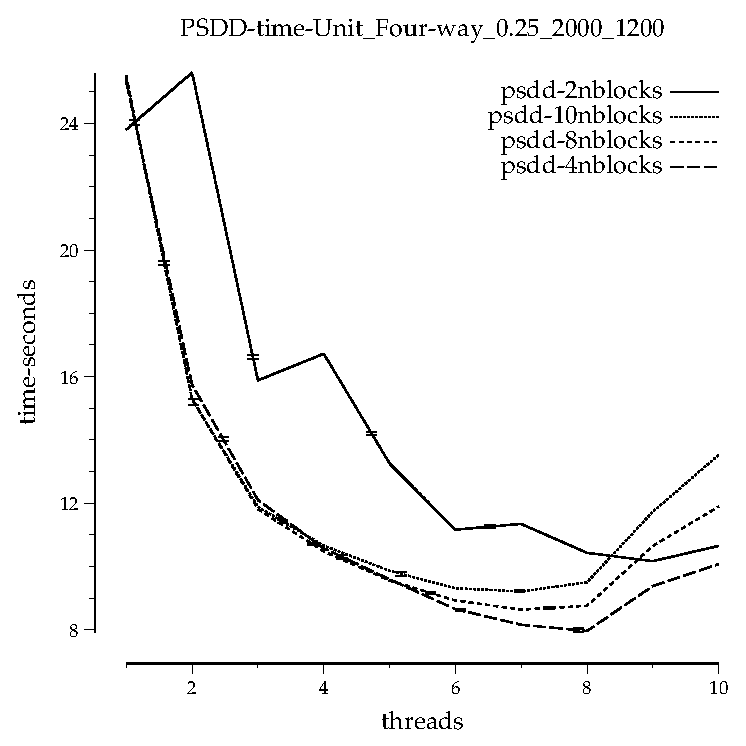
\includegraphics{../graphs/grid_unit_four-way_0.25_2000_1200/PSDD-time-Unit_Four-way_0.25_2000_1200.eps}
\caption{Wall clock time: PSDD on a 2000x1200 grid world with 25\%
  obstacles and unit cost four-way movement.}
\end{center}
\end{figure*}

\begin{figure*}[h]
\begin{center}
\includegraphics[width=3in]{../graphs/grid_unit_four-way_0.25_2000_1200/DYNPSDD-time-Unit_Four-way_0.25_2000_1200_weight=1.1.eps}
\includegraphics[width=3in]{../graphs/grid_unit_four-way_0.25_2000_1200/DYNPSDD-time-Unit_Four-way_0.25_2000_1200_weight=1.5.eps}
\includegraphics[width=3in]{../graphs/grid_unit_four-way_0.25_2000_1200/DYNPSDD-time-Unit_Four-way_0.25_2000_1200_weight=2.0.eps}
\includegraphics[width=3in]{../graphs/grid_unit_four-way_0.25_2000_1200/DYNPSDD-time-Unit_Four-way_0.25_2000_1200_weight=2.2.eps}
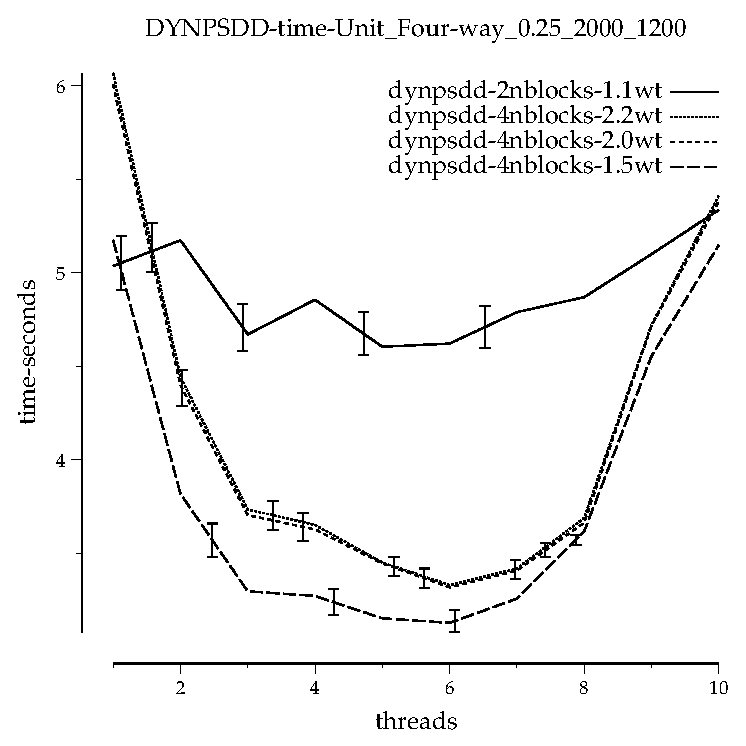
\includegraphics[width=3in]{../graphs/grid_unit_four-way_0.25_2000_1200/DYNPSDD-time-Unit_Four-way_0.25_2000_1200.eps}
\caption{Wall clock time: DYNPSDD on a 2000x1200 grid world with 25\%
  obstacles and unit cost four-way movement.  This algorithm uses wA*
  to get an upper solution cost bound, then performs PSDD using this
  bound for pruning.}
\end{center}
\end{figure*}

\begin{figure*}[h]
\begin{center}
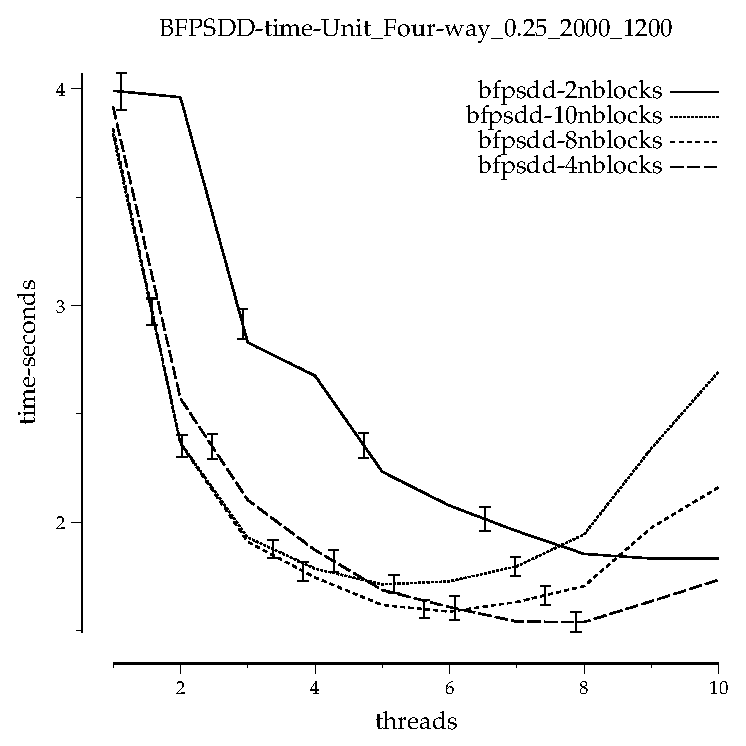
\includegraphics{../graphs/grid_unit_four-way_0.25_2000_1200/BFPSDD-time-Unit_Four-way_0.25_2000_1200.eps}
\caption{Wall clock time: Best-first PSDD on 2000x1200 grid worlds with 25\%
  obstacles and unit cost four-way movement.}
\end{center}
\end{figure*}

\begin{figure*}[h]
\begin{center}
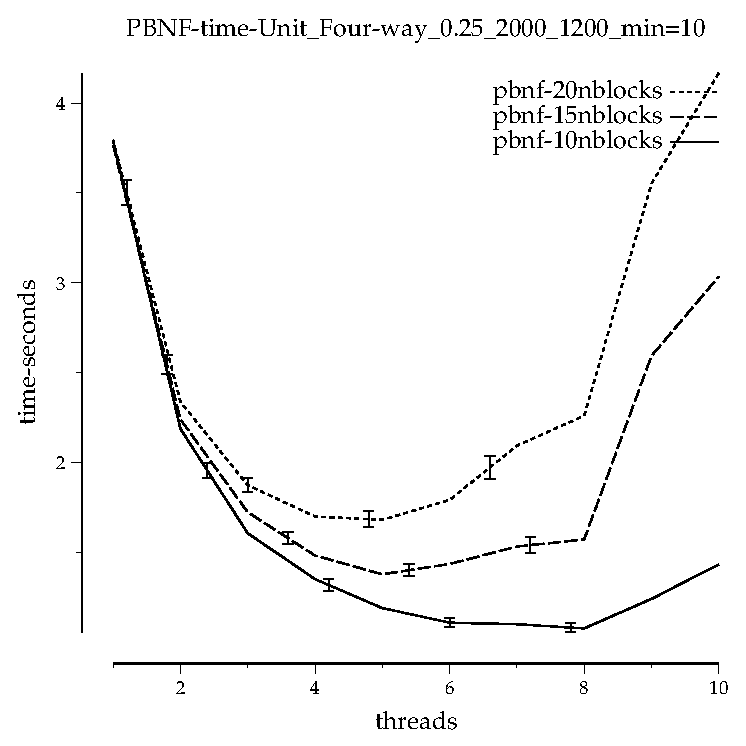
\includegraphics[width=3in]{../graphs/grid_unit_four-way_0.25_2000_1200/PBNF-time-Unit_Four-way_0.25_2000_1200_min=10.eps}
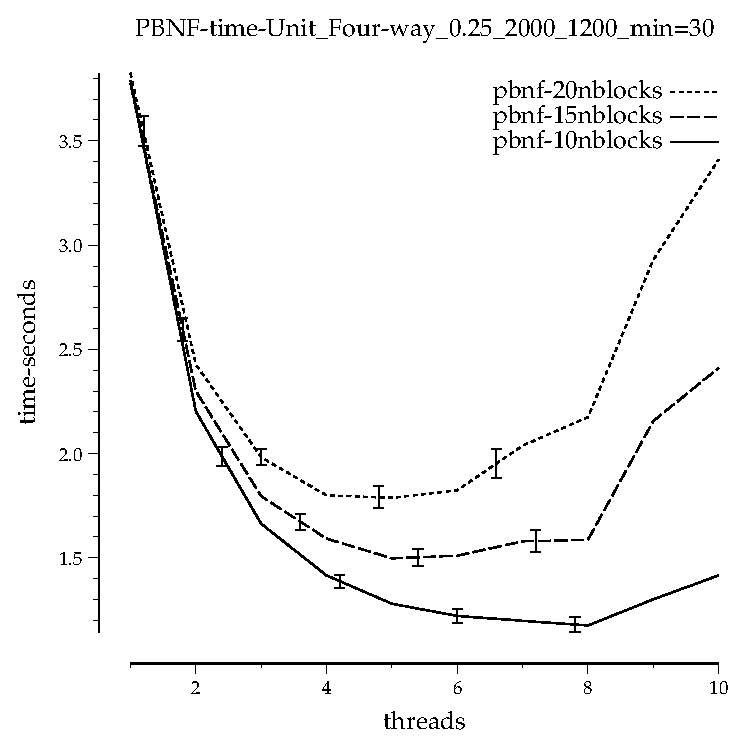
\includegraphics[width=3in]{../graphs/grid_unit_four-way_0.25_2000_1200/PBNF-time-Unit_Four-way_0.25_2000_1200_min=30.eps}
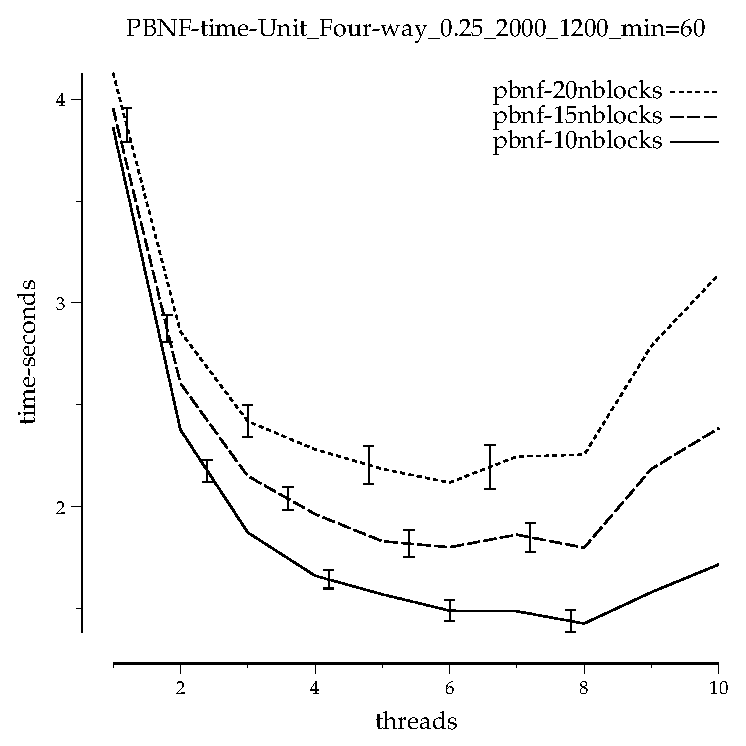
\includegraphics[width=3in]{../graphs/grid_unit_four-way_0.25_2000_1200/PBNF-time-Unit_Four-way_0.25_2000_1200_min=60.eps}
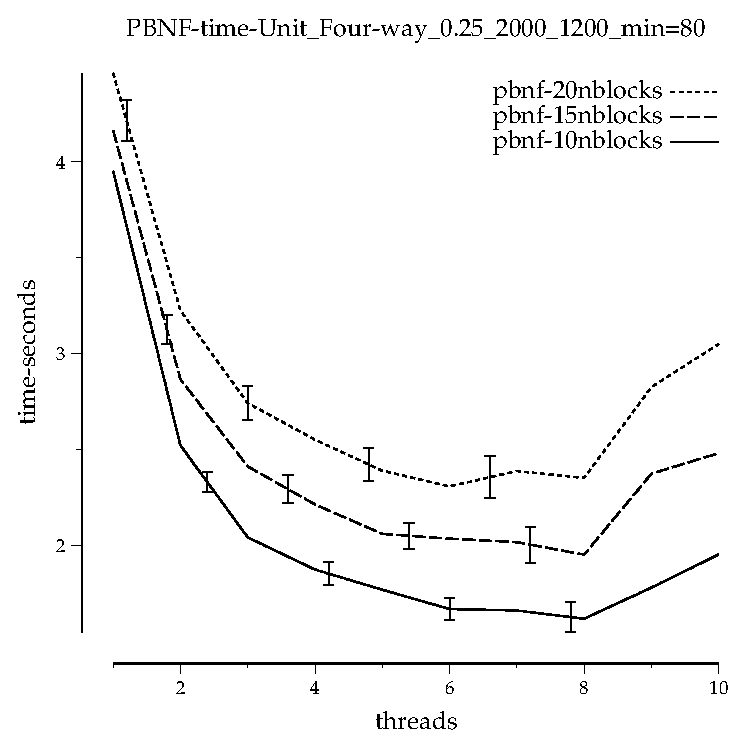
\includegraphics[width=3in]{../graphs/grid_unit_four-way_0.25_2000_1200/PBNF-time-Unit_Four-way_0.25_2000_1200_min=80.eps}
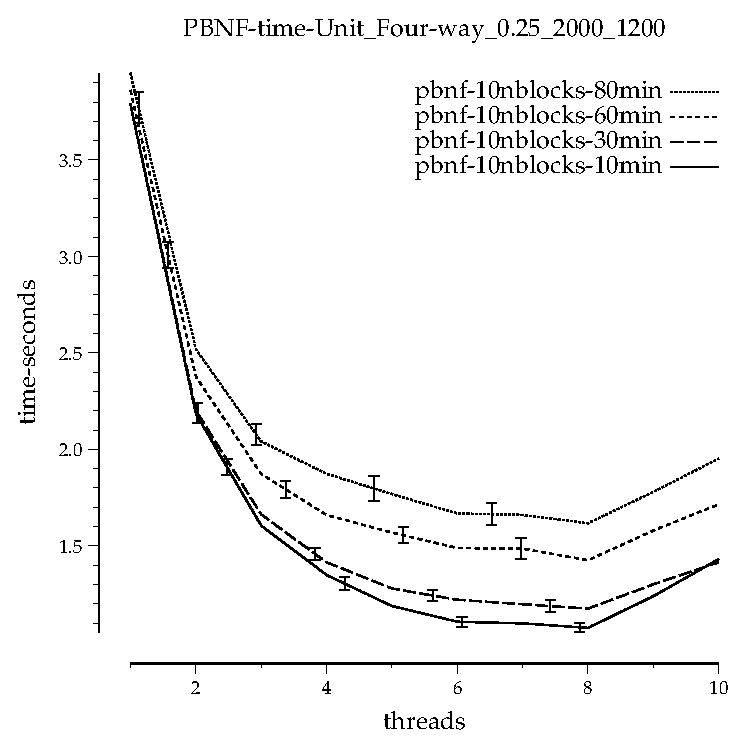
\includegraphics[width=3in]{../graphs/grid_unit_four-way_0.25_2000_1200/PBNF-time-Unit_Four-way_0.25_2000_1200.eps}
\caption{Wall clock time: PBNF on 2000x1200 grid worlds with 25\%
  obstacles and unit cost four-way movement.}
\end{center}
\end{figure*}

\begin{figure*}[h]
\begin{center}
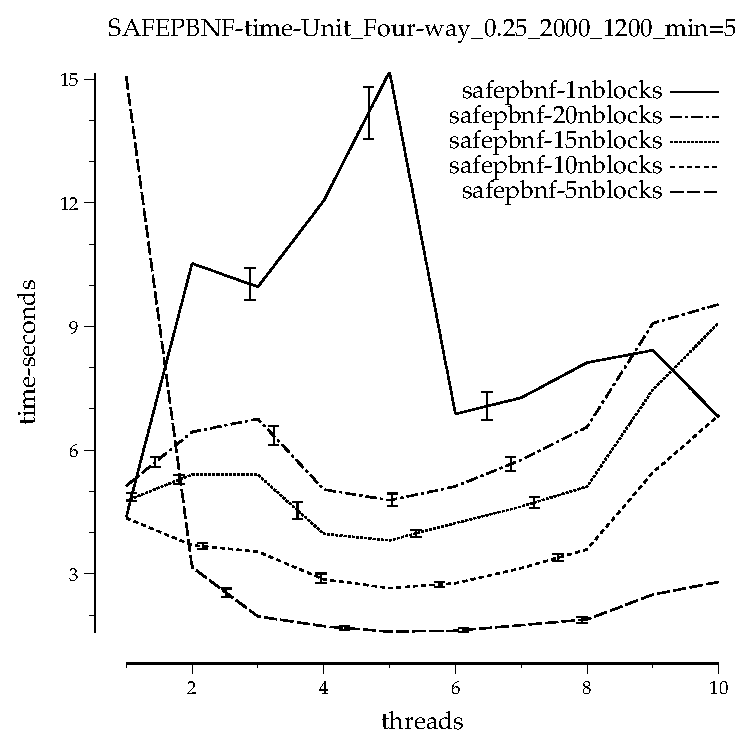
\includegraphics[width=3in]{../graphs/grid_unit_four-way_0.25_2000_1200/SAFEPBNF-time-Unit_Four-way_0.25_2000_1200_min=5.eps}
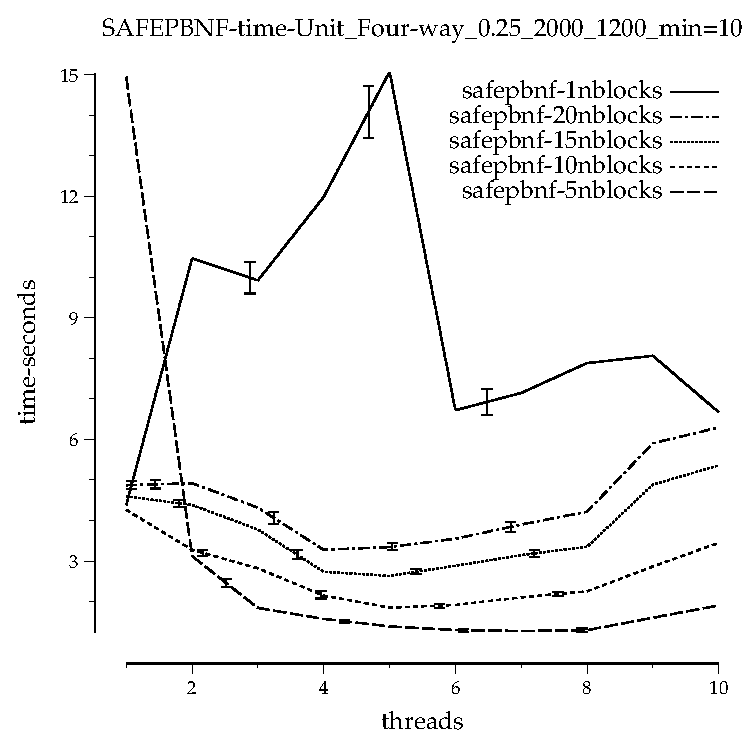
\includegraphics[width=3in]{../graphs/grid_unit_four-way_0.25_2000_1200/SAFEPBNF-time-Unit_Four-way_0.25_2000_1200_min=10.eps}
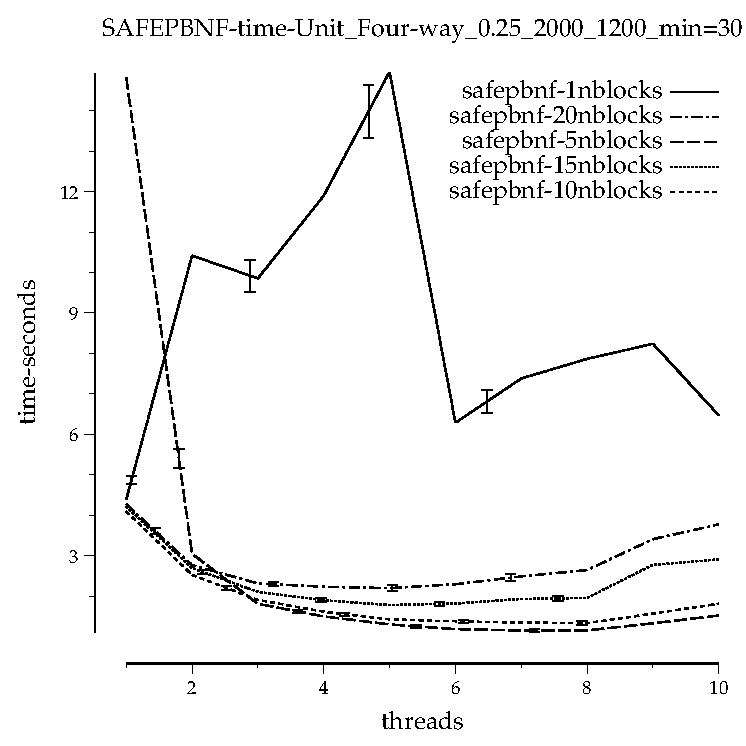
\includegraphics[width=3in]{../graphs/grid_unit_four-way_0.25_2000_1200/SAFEPBNF-time-Unit_Four-way_0.25_2000_1200_min=30.eps}
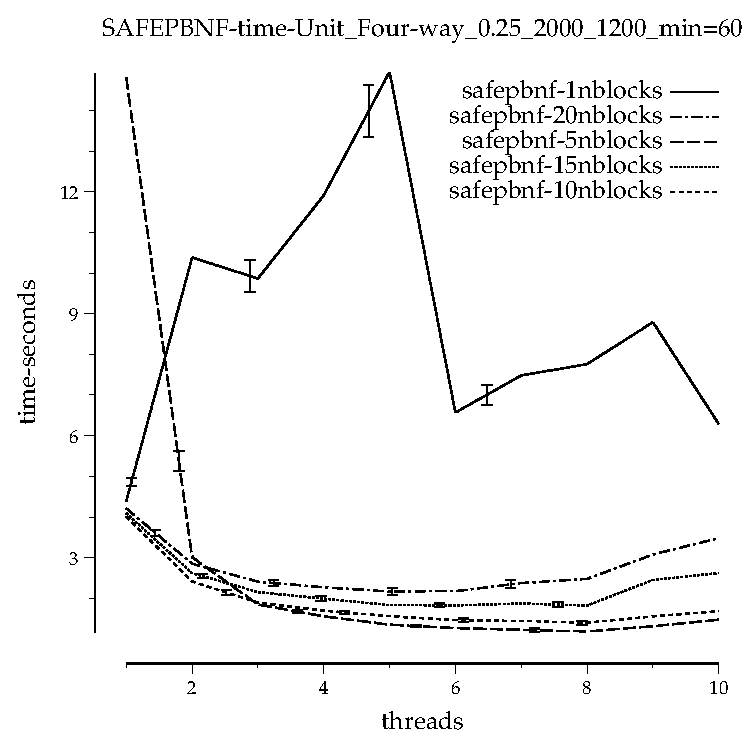
\includegraphics[width=3in]{../graphs/grid_unit_four-way_0.25_2000_1200/SAFEPBNF-time-Unit_Four-way_0.25_2000_1200_min=60.eps}
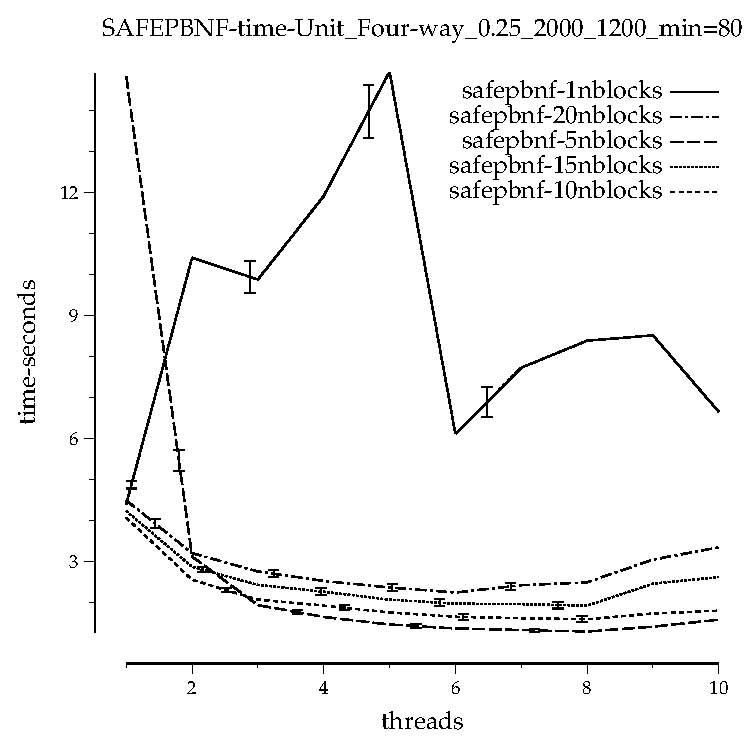
\includegraphics[width=3in]{../graphs/grid_unit_four-way_0.25_2000_1200/SAFEPBNF-time-Unit_Four-way_0.25_2000_1200_min=80.eps}
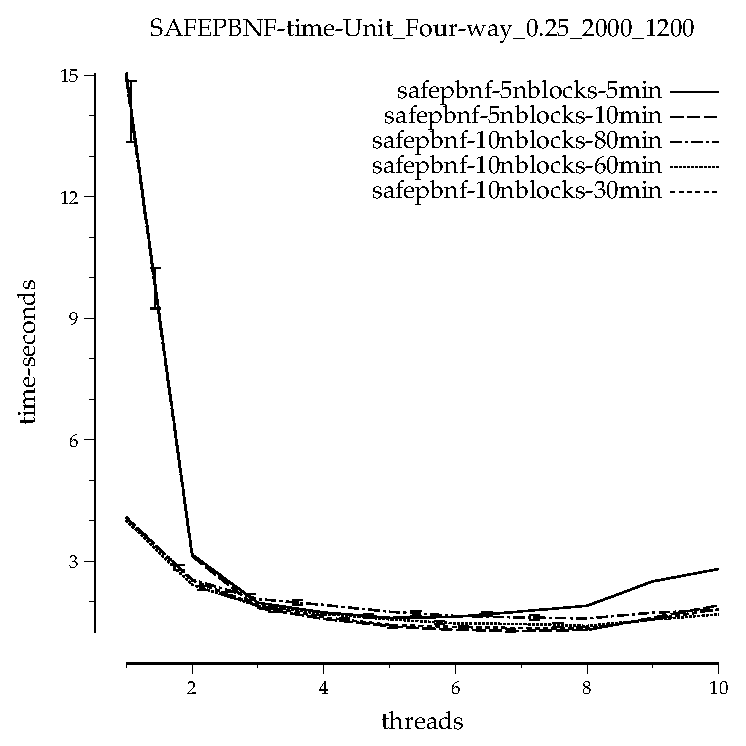
\includegraphics[width=3in]{../graphs/grid_unit_four-way_0.25_2000_1200/SAFEPBNF-time-Unit_Four-way_0.25_2000_1200.eps}
\caption{Wall clock time: Safe PBNF on 2000x1200 grid worlds with 25\%
  obstacles and unit cost four-way movement.}
\end{center}
\end{figure*}

% ------------------------------------------------------------

\begin{figure*}[h]
\begin{center}
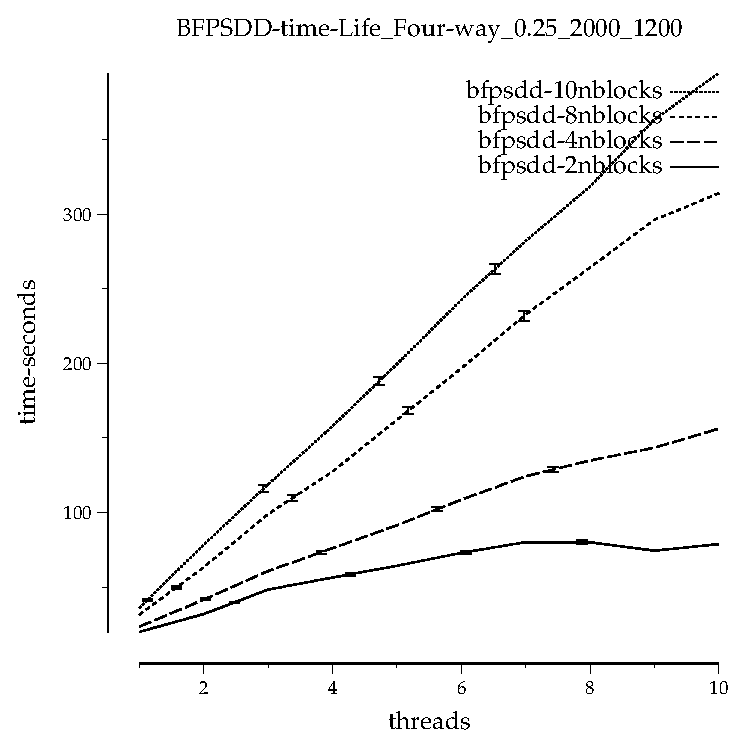
\includegraphics{../graphs/grid_life_four-way_0.25_2000_1200/BFPSDD-time-Life_Four-way_0.25_2000_1200.eps}
\caption{Wall clock time: Best-first PSDD on 2000x1200 grid worlds with 25\%
  obstacles and life cost four-way movement.}
\end{center}
\end{figure*}

\begin{figure*}[h]
\begin{center}
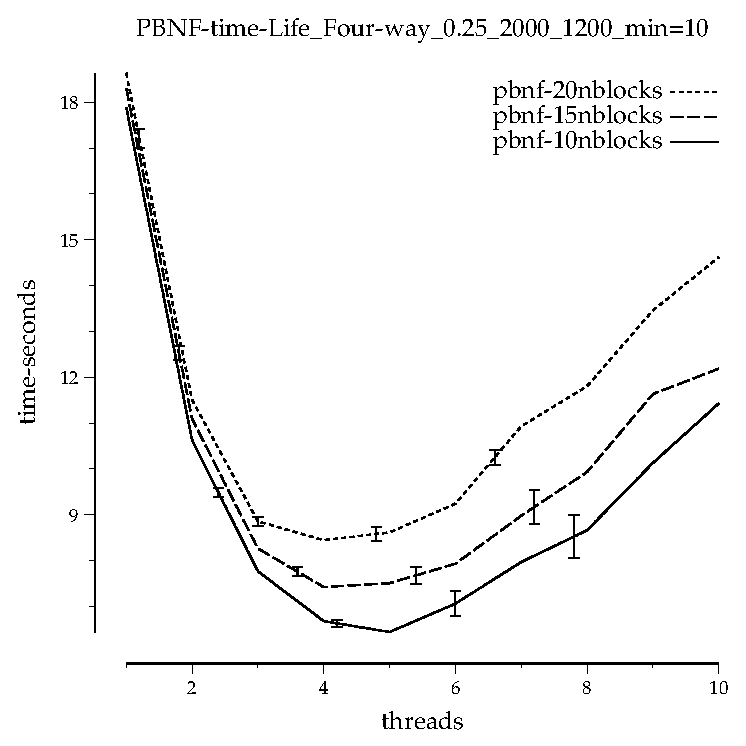
\includegraphics[width=3in]{../graphs/grid_life_four-way_0.25_2000_1200/PBNF-time-Life_Four-way_0.25_2000_1200_min=10.eps}
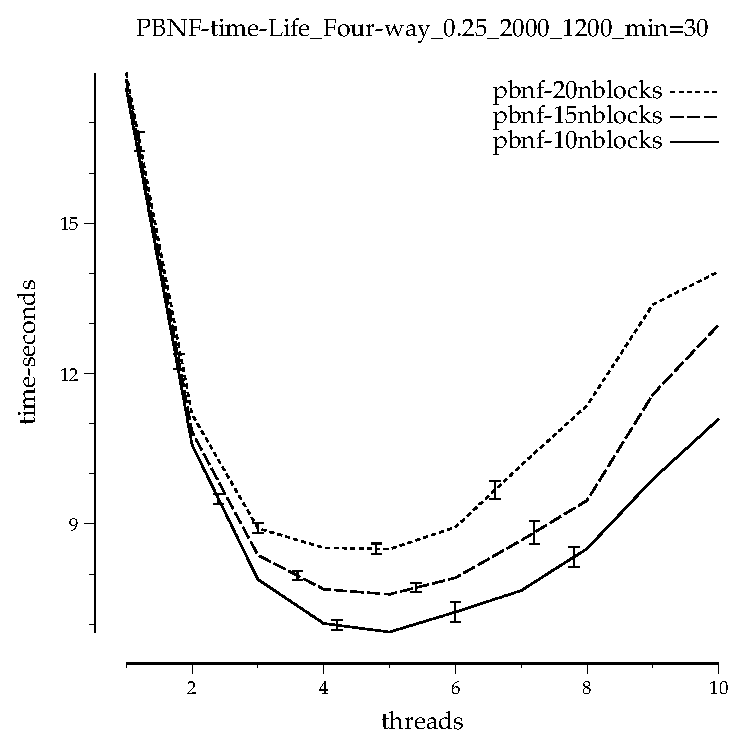
\includegraphics[width=3in]{../graphs/grid_life_four-way_0.25_2000_1200/PBNF-time-Life_Four-way_0.25_2000_1200_min=30.eps}
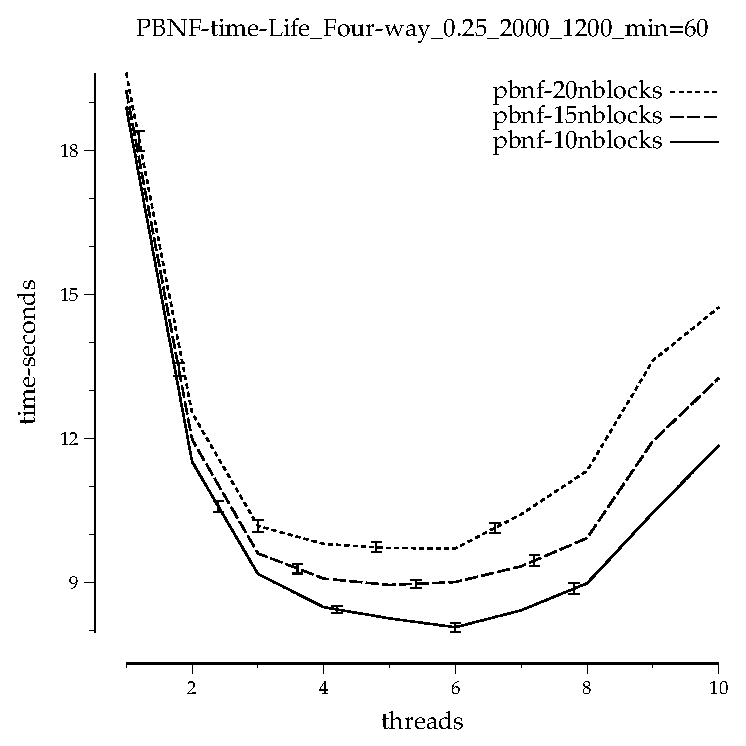
\includegraphics[width=3in]{../graphs/grid_life_four-way_0.25_2000_1200/PBNF-time-Life_Four-way_0.25_2000_1200_min=60.eps}
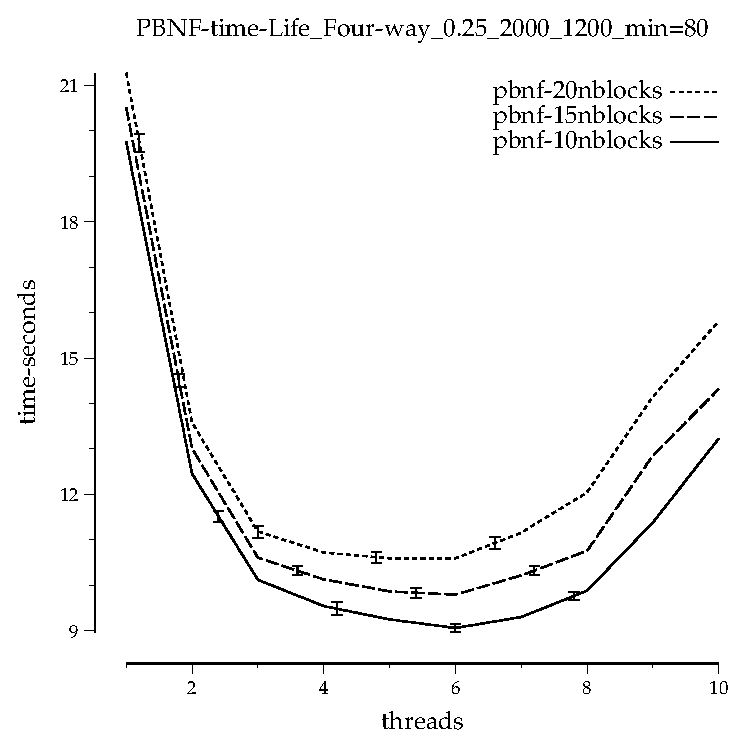
\includegraphics[width=3in]{../graphs/grid_life_four-way_0.25_2000_1200/PBNF-time-Life_Four-way_0.25_2000_1200_min=80.eps}
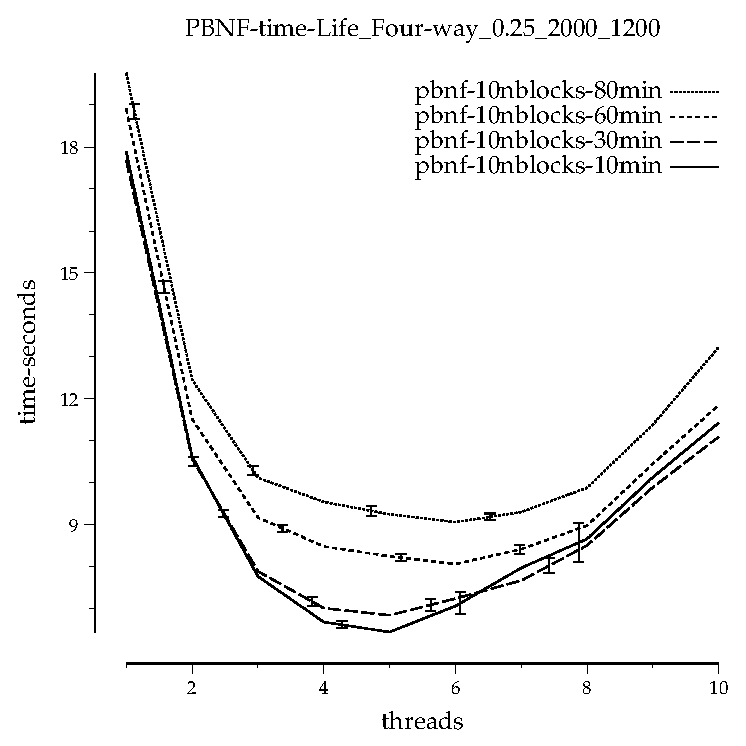
\includegraphics[width=3in]{../graphs/grid_life_four-way_0.25_2000_1200/PBNF-time-Life_Four-way_0.25_2000_1200.eps}
\caption{Wall clock time: PBNF on 2000x1200 grid worlds with 25\%
  obstacles and life cost four-way movement.}
\end{center}
\end{figure*}

\begin{figure*}[h]
\begin{center}
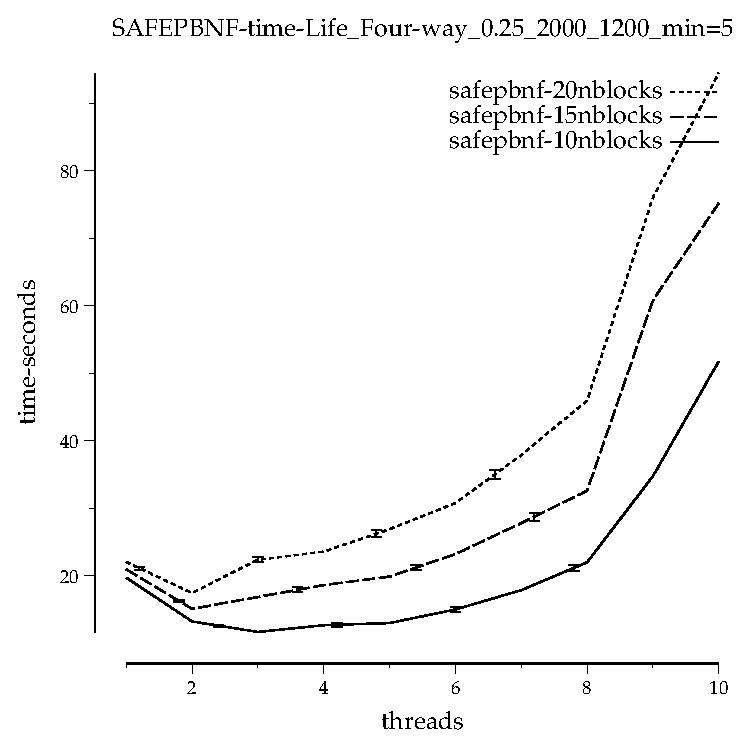
\includegraphics[width=3in]{../graphs/grid_life_four-way_0.25_2000_1200/SAFEPBNF-time-Life_Four-way_0.25_2000_1200_min=5.eps}
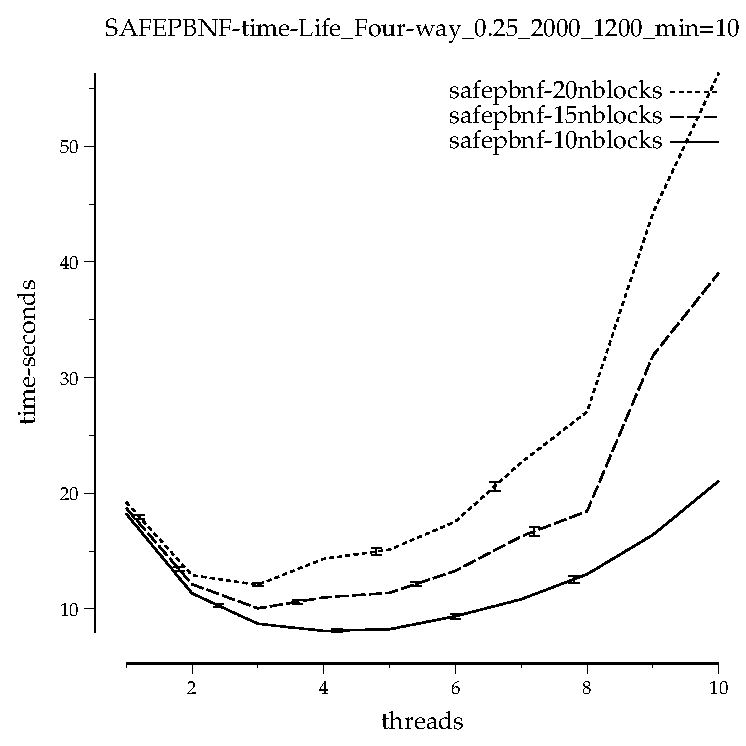
\includegraphics[width=3in]{../graphs/grid_life_four-way_0.25_2000_1200/SAFEPBNF-time-Life_Four-way_0.25_2000_1200_min=10.eps}
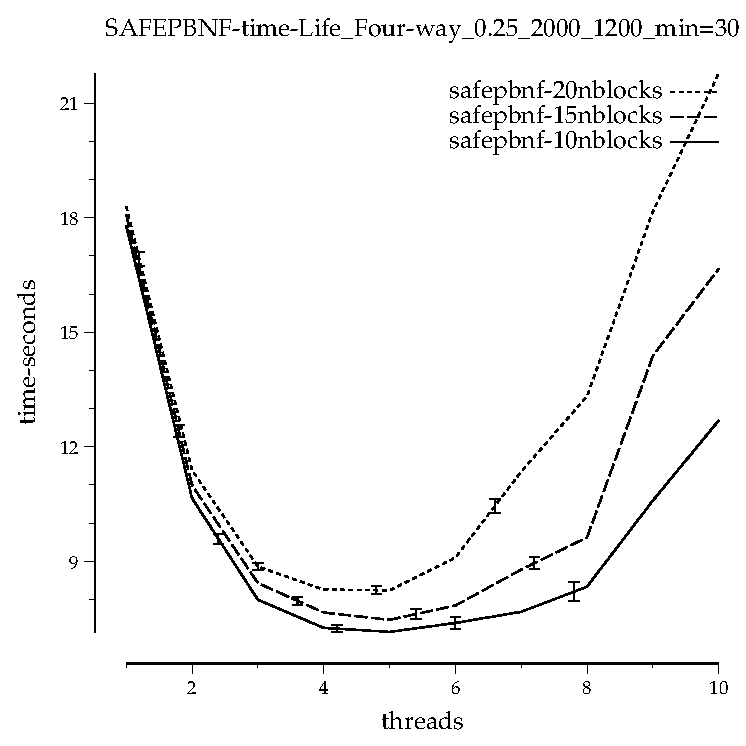
\includegraphics[width=3in]{../graphs/grid_life_four-way_0.25_2000_1200/SAFEPBNF-time-Life_Four-way_0.25_2000_1200_min=30.eps}
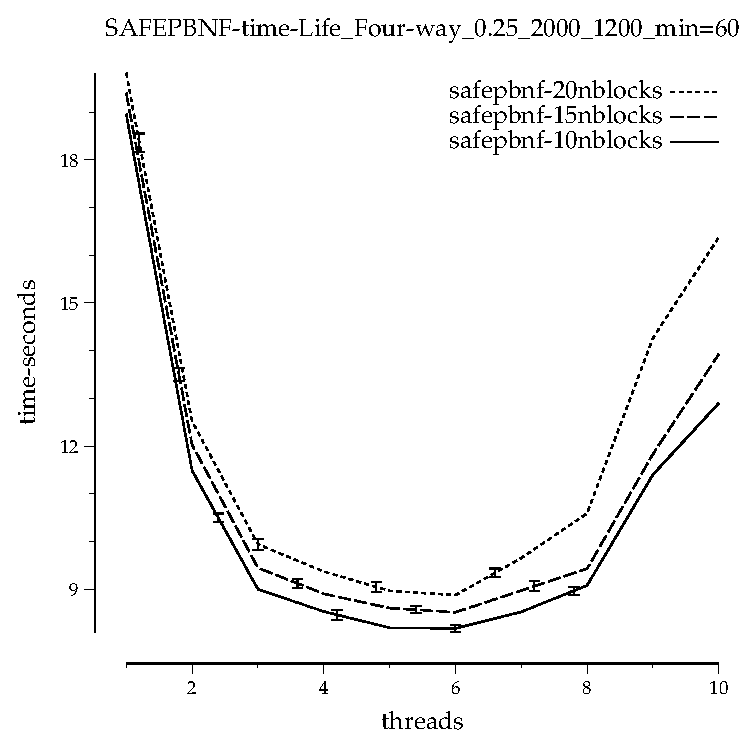
\includegraphics[width=3in]{../graphs/grid_life_four-way_0.25_2000_1200/SAFEPBNF-time-Life_Four-way_0.25_2000_1200_min=60.eps}
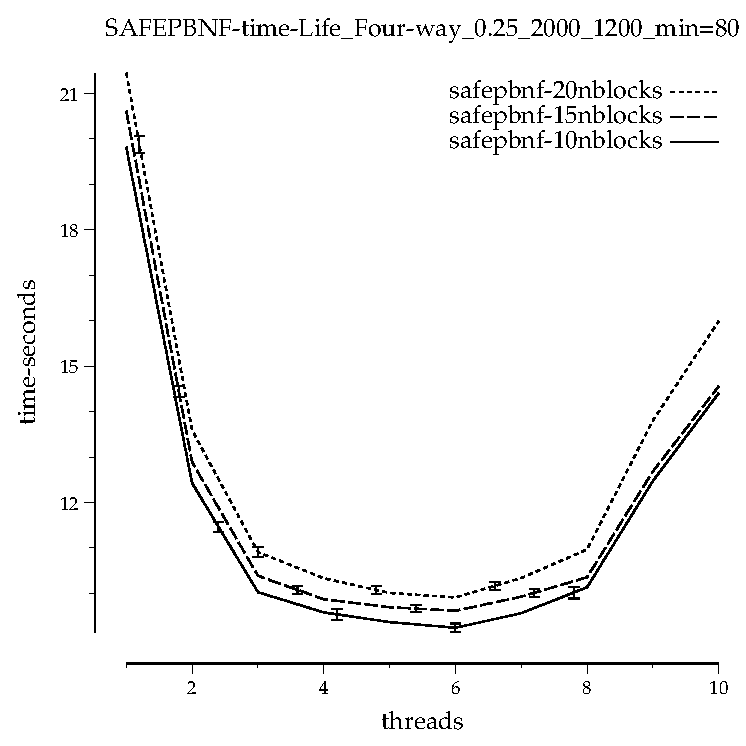
\includegraphics[width=3in]{../graphs/grid_life_four-way_0.25_2000_1200/SAFEPBNF-time-Life_Four-way_0.25_2000_1200_min=80.eps}
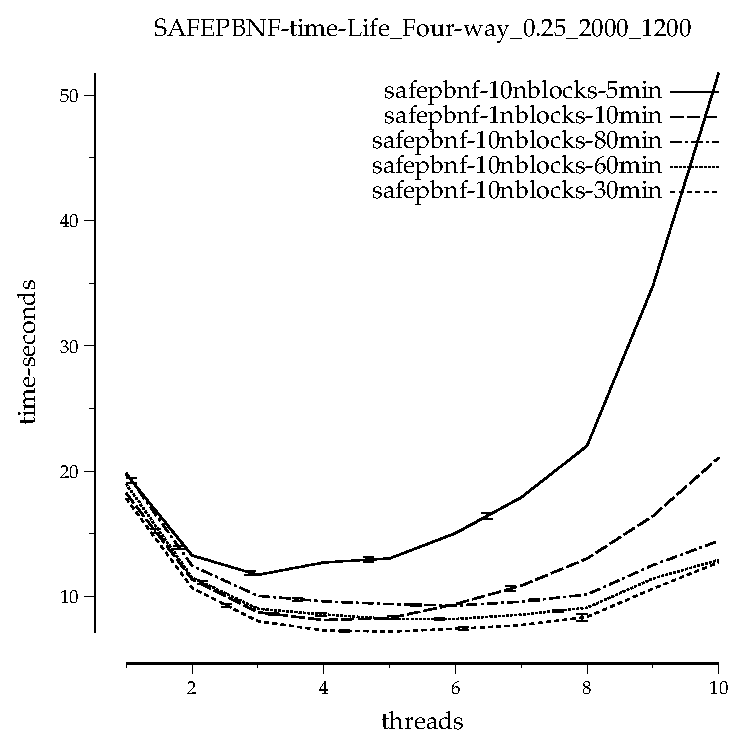
\includegraphics[width=3in]{../graphs/grid_life_four-way_0.25_2000_1200/SAFEPBNF-time-Life_Four-way_0.25_2000_1200.eps}
\caption{Wall clock time: Safe PBNF on 2000x1200 grid worlds with 25\%
  obstacles and life cost four-way movement.}
\end{center}
\end{figure*}

% ------------------------------------------------------------

\begin{figure*}[h]
\begin{center}
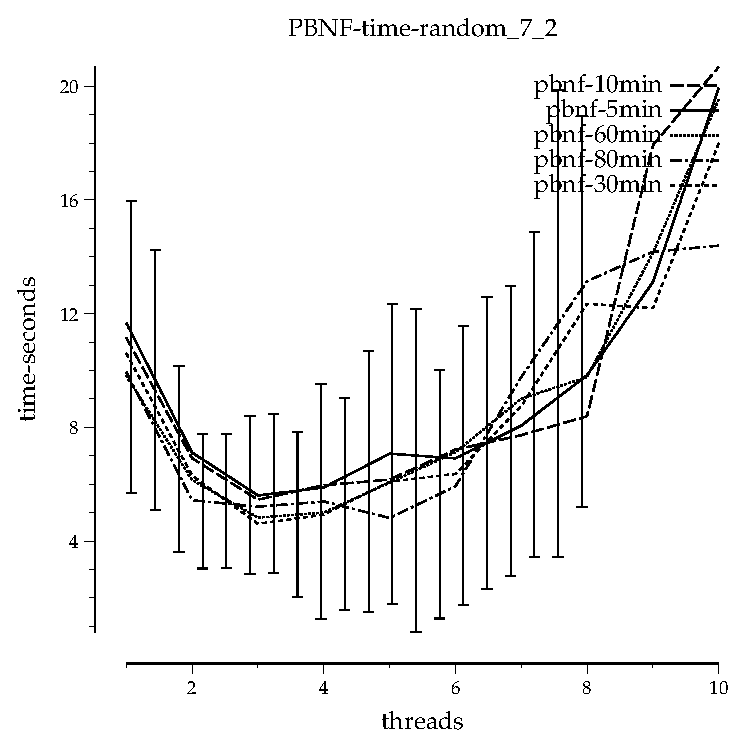
\includegraphics[width=3in]{../graphs/tiles_random_7_2/PBNF-time-random_7_2.eps}
\caption{Wall clock time: PBNF on random 7x2 tiles puzzles.}
\end{center}
\end{figure*}

\begin{figure*}[h]
\begin{center}
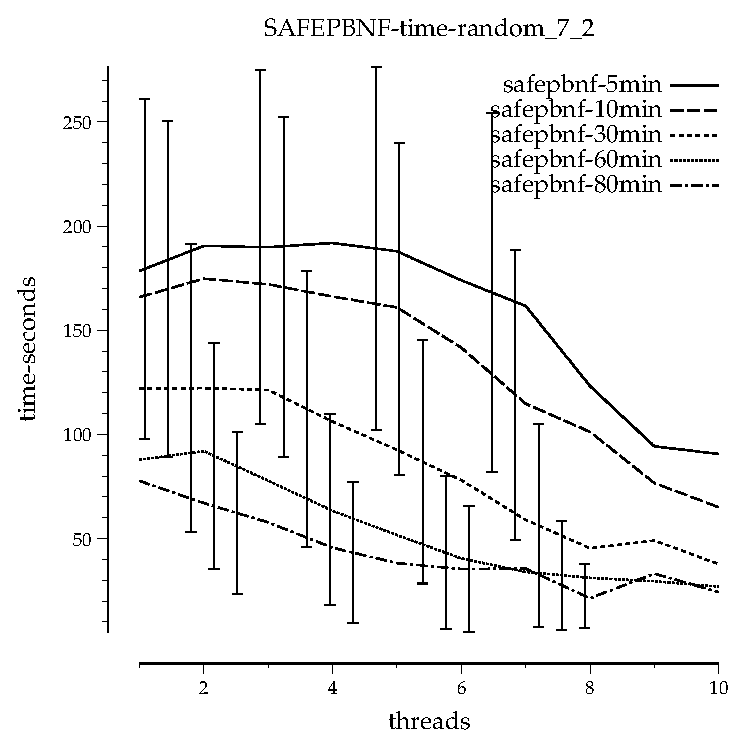
\includegraphics[width=3in]{../graphs/tiles_random_7_2/SAFEPBNF-time-random_7_2.eps}
\caption{Wall clock time: Safe PBNF on random 7x2 tiles puzzles.}
\end{center}
\end{figure*}

% ------------------------------------------------------------
% ------------------------------------------------------------
% ------------------------------------------------------------

\end{appendices}

\end{document}
